% !TEX program = xelatex
\documentclass[UTF8,fontset=fandol,a4paper,11pt]{ctexart}
\usepackage[margin=21mm,top=23mm,bottom=22mm,headheight=16pt]{geometry}
\usepackage{amsmath,amssymb,mathtools,bm}
\usepackage{tikz}
\usetikzlibrary{arrows.meta,calc,angles,quotes,patterns}
\usepackage{xcolor,booktabs,array,longtable,enumitem,fancyhdr,needspace}
\usepackage[unicode,hidelinks]{hyperref}
\definecolor{ink}{HTML}{24343C}
\definecolor{accent}{HTML}{166A70}
\definecolor{muted}{HTML}{65747A}
\definecolor{rulegray}{HTML}{D4DDE0}
\definecolor{warm}{HTML}{966037}
\color{ink}
\setlength{\parindent}{2em}
\setlength{\parskip}{4pt}
\linespread{1.12}
\AtBeginDocument{\setlength{\abovedisplayskip}{6pt plus 2pt minus 1pt}
\setlength{\belowdisplayskip}{6pt plus 2pt minus 1pt}
\setlength{\abovedisplayshortskip}{0pt plus 1pt}
\setlength{\belowdisplayshortskip}{4pt plus 1pt}}
\setlist[enumerate]{label=(\arabic*),leftmargin=2.3em,itemsep=3pt,topsep=4pt}
\setlist[itemize]{leftmargin=2em,itemsep=2pt,topsep=4pt}
\allowdisplaybreaks[1]
\setlength{\emergencystretch}{2em}
\setcounter{secnumdepth}{0}
\providecommand{\tightlist}{\setlength{\itemsep}{0pt}\setlength{\parskip}{0pt}}
\ctexset{section={format=\Large\bfseries\color{accent},beforeskip=10pt,afterskip=9pt},
subsection={format=\normalsize\bfseries\color{accent},beforeskip=10pt,afterskip=4pt},
subsubsection={format=\normalsize\bfseries,beforeskip=8pt,afterskip=3pt}}
\pagestyle{fancy}
\fancyhf{}
\fancyhead[L]{\small\color{muted}物理学难题集萃}
% 页眉仅保留书名；版本名称只在封面显示。
\fancyfoot[L]{\small\color{muted}\chapterlabel}
\fancyfoot[R]{\small\thepage}
\renewcommand{\headrulewidth}{0.4pt}
\renewcommand{\footrulewidth}{0pt}
\newcommand{\dd}{\mathop{}\!\mathrm{d}}
\newcommand{\vect}[1]{\bm{#1}}
\newcommand{\tagline}[1]{\noindent{\small\color{muted}#1}\par}
\newcommand{\result}[1]{\begin{equation*}\boxed{#1}\end{equation*}}
\newcommand{\figcaption}[1]{\par\vspace{2pt}{\small\color{muted}#1}\par}
\newcommand{\teach}[2]{\Needspace{4\baselineskip}\subsection*{讲解要点与追问}#1\par\smallskip\noindent\textbf{追问：}#2\par}
\newcommand{\workarea}{\par\vspace{7mm}\noindent{\small\color{muted}作答区}\par\vspace{4mm}
\noindent\textcolor{rulegray}{\rule{\linewidth}{0.3pt}}\par\vspace{16mm}
\noindent\textcolor{rulegray}{\rule{\linewidth}{0.3pt}}\par\vspace{16mm}
\noindent\textcolor{rulegray}{\rule{\linewidth}{0.3pt}}\par\vspace{16mm}
\noindent\textcolor{rulegray}{\rule{\linewidth}{0.3pt}}}
\tikzset{axis/.style={-{Stealth[length=2mm]},thin,color=muted},
motion/.style={-{Stealth[length=2.3mm]},thick,color=accent},
force/.style={-{Stealth[length=2.3mm]},thick,color=warm},
traj/.style={thick,color=accent},guide/.style={dashed,thin,color=muted},
object/.style={thick,color=ink},every node/.style={font=\small}}\widowpenalty=10000\clubpenalty=10000\displaywidowpenalty=10000\newcommand{\chapterlabel}{电磁学试题（二）}







\hypersetup{pdftitle={电磁学试题（二）·学生解答版},pdfauthor={}}

\begin{document}\pdfbookmark[0]{电磁学试题（二）}{cover}

\thispagestyle{empty}\vspace*{22mm}

\noindent{\Huge\bfseries 物理学难题集萃}\par\vspace{12mm}

\noindent{\LARGE 电磁学试题（二）}\par\vspace{12mm}

\noindent{\Large\color{accent}学生解答版}\par\vspace{9mm}

\noindent\textcolor{accent}{\rule{\linewidth}{1pt}}\par\vspace{9mm}

\noindent 第1--5题\par\vfill\clearpage

\pdfbookmark[1]{题目目录}{contents}\section*{题目目录}

\begin{longtable}{@{}r p{113mm} r@{}}\toprule 题号 & 题目 & 页码\\\midrule

\hyperref[q:1]{1} & \hyperref[q:1]{带电圆环中心附近的受限小振动} & \pageref{q:1} \\

\hyperref[q:2]{2} & \hyperref[q:2]{圆锥曲线电流在焦点处的磁场} & \pageref{q:2} \\

\hyperref[q:3]{3} & \hyperref[q:3]{磁力辅助的圆环外侧持续绕行} & \pageref{q:3} \\

\hyperref[q:4]{4} & \hyperref[q:4]{匀强磁场中电阻网络的总安培力} & \pageref{q:4} \\

\hyperref[q:5]{5} & \hyperref[q:5]{时变磁场中带电弦杆的转动与端点作用力} & \pageref{q:5} \\

\bottomrule\end{longtable}

\clearpage

\pdfbookmark[2]{第 1 题 带电圆环中心附近的受限小振动}{q1}

\section*{第 1 题\quad 带电圆环中心附近的受限小振动}\label{q:1}


线电荷密度为$\lambda>0$、半径为$R$的均匀带电圆环，固定在光滑的水平绝缘桌面上。质量为$m$、电荷为$q>0$的小球静止释放于桌面内距环心$O$为$r_0\ll R$处。圆环电荷分布不受小球影响，忽略辐射。
判断小球是否振动，并用有物理依据的近似方法估算周期。说明近似适用条件，以及桌面对运动的限制为何必要。


\begin{center}\begin{minipage}{.98\linewidth}\centering
\begin{tikzpicture}[scale=.9,transform shape]

\draw[object] (0,0) circle (2);
\draw[axis] (-2.7,0)--(3.1,0) node[right] {$x$};
\fill (0,0) circle (1.6pt) node[below left] {$O$};
\fill[color=accent] (.7,0) circle (2.5pt) node[above right] {$P_0:m,q$};
\draw[guide] (0,0)--(-1.414,-1.414) node[midway,above left] {$R$};
\draw[axis,<->] (0,-.5)--(.7,-.5) node[midway,below] {$r_0$};
\node at (0,2.5) {均匀正电环 $\lambda>0$};
\node at (0,-2.7) {水平面俯视；静止释放};

\end{tikzpicture}
\figcaption{图电试2.1\quad 圆环与小球同在桌面内，初始偏离中心很小。}
\end{minipage}\end{center}

\Needspace{6\baselineskip}\subsection*{解答}


图电试2.1中小球从$P_0$静止释放。圆环电场在桌面内沿径向，初始角动量为零，此后小球始终沿$OP_0$这一直径运动。用有正负的$x$表示直径坐标，小球通过环心时$x$连续变号，径向距离则为$r=|x|$。

环心处由对径电荷元的电场相消而有$\boldsymbol E=0$，但稳定性由小位移后的场决定。小球偏离中心时，环上近、远两侧电荷既有不同距离，也有不同的电场投影，合场的方向由整环叠加决定。利用圆环的转动对称和中心附近没有环上电荷的性质，可以把面内场与较容易计算的轴线场联系起来。先算与圆环垂直的$z$轴上的电场。总电荷$Q_{\rm ring}=2\pi R\lambda$，对称性使横向分量相消，故
\[
E_z(0,z)=\frac{1}{4\pi\varepsilon_0}
\frac{Q_{\rm ring}z}{(R^2+z^2)^{3/2}}
=a z[1+O(z^2/R^2)],\qquad
a=\frac{\lambda}{2\varepsilon_0R^2}.
\]
轴线上每个电荷元到观察点的距离同为$\sqrt{R^2+z^2}$，电场在轴向的投影因子为$z/\sqrt{R^2+z^2}$，所以精确分母为$(R^2+z^2)^{3/2}$。中心附近展开$[1+(z/R)^2]^{-3/2}$，主项是正的一阶系数$a$，首个略去项为$-3az^3/(2R^2)$。轴向场在中心两侧都指向外，桌面内的径向场随后由同一局部区域的电通量求出。
\begin{center}\begin{minipage}{.98\linewidth}\centering
\begin{tikzpicture}[scale=.85,transform shape]

\draw[axis] (-3.2,0)--(3.2,0) node[right] {$z$};
\draw[object] (-1.3,-.7) rectangle (1.3,.7);
\draw[guide] (-1.3,-.7) arc[start angle=-90,end angle=90,x radius=.2,y radius=.7];
\draw[object] (1.3,-.7) arc[start angle=-90,end angle=90,x radius=.2,y radius=.7];
\node[below left] at (0,0) {$O$};
\draw[motion] (1.3,.35)--(2.5,.35) node[right] {$+ah$};
\draw[motion] (-1.3,.35)--(-2.5,.35) node[left] {$-ah$};
\draw[force] (0,1.5)--(0,.7) node[midway,right] {$E_\rho<0$};
\draw[force] (0,-1.5)--(0,-.7);
\draw[axis,<->] (-1.3,-1.9)--(1.3,-1.9) node[midway,below] {$2h$};
\draw[axis,<->] (.6,0)--(.6,.7) node[midway,right] {$\rho$};
\node at (0,2.15) {轴向剖面：端面出流，侧面入流};

\end{tikzpicture}
\figcaption{解图电试2.1A\quad 小柱无包围电荷，两端正通量与侧面负通量相抵。}
\end{minipage}\end{center}
解图电试2.1A以$O$为中心取半径$\rho$、高$2h$的小圆柱，$\rho,h\ll R$。柱内没有圆环上的电荷，高斯定理要求总电通量为零。两端面的外法线分别沿$\pm z$，两端通量同为正；保留一阶场，
\[
\Phi_{\rm end}\simeq2\pi\rho^2 ah,\qquad
\Phi_{\rm side}\simeq(2\pi\rho)(2h)E_\rho.
\]
上端面有$E_z\simeq+ah$和外法线$+\hat z$，下端面有$E_z\simeq-ah$和外法线$-\hat z$，两次点乘均为正。每端面积$\pi\rho^2$，两端合计$2\pi\rho^2$；侧面面积为周长$2\pi\rho$乘高度$2h$。轴对称使侧面的一阶径向场沿圆周相同，关于中平面的对称又使它在高度方向的一阶变化消失。由$\Phi_{\rm end}+\Phi_{\rm side}=0$，
\[
\boxed{E_\rho\simeq-\frac a2\rho
=-\frac{\lambda}{4\varepsilon_0R^2}\rho}.
\]
负号说明桌面内电场指向$O$，同号带电小球在环内中心附近受到恢复力。小柱通量保留局部场的一阶项，有限柱面上的场强变化进入更高阶项；令柱的各尺度相对环半径变小，得到上述确定的一阶系数。

具体地，局部轴对称场可写$E_\rho=b\rho+O[a\rho(\rho^2+z^2)/R^2]$、$E_z=az+O[az(\rho^2+z^2)/R^2]$。保留一阶后，总通量与$2b+a$成正比，故$b=-a/2$。这给出确定的局部恢复刚度，而柱面上的场在有限尺寸下仍随位置变化。取$\rho,h$同阶且都远小于$R$，这些变化相对主项均为小量。

中心电场的力矩为零，保持了静止释放时的零角动量。桌面内的径向轨迹沿初始直径延伸，速度指向或背离环心，过中心后继续走向另一侧。重力与桌面支持力在竖直方向平衡，面内动力学只包含圆环的静电力。在直径上写成
\[
m\ddot x=-\frac{\lambda q}{4\varepsilon_0R^2}x,\qquad
\omega^2=\frac{\lambda q}{4\varepsilon_0mR^2}.
\]
用$x(0)=r_0,\dot x(0)=0$，
\[
\boxed{x(t)\simeq r_0\cos\omega t,\qquad
T\simeq4\pi R\sqrt{\frac{\varepsilon_0m}{\lambda q}}}.
\]
\begin{center}\begin{minipage}{.98\linewidth}\centering
\begin{tikzpicture}[scale=.8,transform shape]

\draw[axis] (-2.6,0)--(2.7,0) node[right] {$x/r_0$};
\draw[axis] (0,-.25)--(0,2.6) node[above] {$\displaystyle\frac{U-U(0)}{m\omega^2 r_0^2/2}$};
\draw[traj,domain=-1.55:1.55,samples=60] plot (\x,{\x*\x});
\draw[guide] (-1,0)--(-1,1)--(1,1)--(1,0);
\draw[object] (-.055,1)--(.055,1) node[above right] {$1$};
\node[below] at (-1,0) {$-1$};\node[below] at (1,0) {$1$};
\node[below left] at (0,0) {$O$};
\draw[motion] (1,.35)--(.35,.35);
\draw[motion] (-1,.35)--(-.35,.35);
\begin{scope}[xshift=5.7cm]
\draw[axis] (-1.5,0)--(1.6,0) node[right] {$\delta z$};
\fill (0,0) circle (1.5pt);
\draw[force] (.35,0)--(1.15,0);
\draw[force] (-.35,0)--(-1.15,0);
\node at (0,1.1) {轴向轨迹间距增长};
\node at (0,-1) {$m\delta\ddot z=qa\delta z$};
\end{scope}

\end{tikzpicture}
\figcaption{解图电试2.1B\quad 左图的面内势能取二次项；右图箭头表示两条轴向轨迹的电场力差。}
\end{minipage}\end{center}
解图电试2.1B的势能曲线在$x=0$处有极小值，两侧转折点为$\pm r_0$。势能曲率与振幅修正可由圆环电势在桌面内的展开求出：
\[
V(x)=\frac{\lambda}{4\pi\varepsilon_0}
\int_0^{2\pi}\frac{d\varphi}
{\sqrt{1-2(x/R)\cos\varphi+(x/R)^2}}
=\frac{\lambda}{2\varepsilon_0}
\left[1+\frac{x^2}{4R^2}
+\frac{9x^4}{64R^4}+O(x^6/R^6)\right].
\]
展开积分时令$s=x/R$，被积函数的一次项含$\cos\varphi$，对整环积分为零；二次平均含$\langle\cos^2\varphi\rangle=1/2$，得到$s^2/4$。关于环心反演的对称性消去所有奇次势能项，所以恢复力的下一项是三次项。势能$\mathcal U=qV$的二次部分为$\lambda qx^2/(8\varepsilon_0R^2)=m\omega^2x^2/2$，在图B的中心向两侧升高，两转折点具有相同的总能量。二次项求导给出同一恢复力；首个非线性修正相对为$O(r_0^2/R^2)$，所以周期估算的误差也为这一阶。较大振幅的周期由完整电势的能量积分计算。

\begin{center}\begin{minipage}{.98\linewidth}\centering
\begin{tikzpicture}[scale=.8,transform shape]
\draw[axis] (0,0)--(10.7,0) node[right] {$x/R$};
\draw[axis] (0,0)--(0,3.2) node[above] {$qE_x/(m\omega^2R)$};
\node[above] at (5,3.5) {实线完整库仑积分，虚线近中心线性恢复场};
\draw[traj] plot coordinates {(0.000000000,2.567286766) (0.083333333,2.543641126) (0.166666667,2.520233916) (0.250000000,2.497058545) (0.333333333,2.474108585) (0.416666667,2.451377768) (0.500000000,2.428859975) (0.583333333,2.406549234) (0.666666667,2.384439714) (0.750000000,2.362525720) (0.833333333,2.340801684) (0.916666667,2.319262166) (1.000000000,2.297901846) (1.083333333,2.276715520) (1.166666667,2.255698095) (1.250000000,2.234844587) (1.333333333,2.214150114) (1.416666667,2.193609895) (1.500000000,2.173219243) (1.583333333,2.152973565) (1.666666667,2.132868356) (1.750000000,2.112899195) (1.833333333,2.093061746) (1.916666667,2.073351749) (2.000000000,2.053765021) (2.083333333,2.034297451) (2.166666667,2.014944999) (2.250000000,1.995703692) (2.333333333,1.976569618) (2.416666667,1.957538933) (2.500000000,1.938607846) (2.583333333,1.919772626) (2.666666667,1.901029595) (2.750000000,1.882375128) (2.833333333,1.863805649) (2.916666667,1.845317628) (3.000000000,1.826907582) (3.083333333,1.808572071) (3.166666667,1.790307695) (3.250000000,1.772111092) (3.333333333,1.753978939) (3.416666667,1.735907946) (3.500000000,1.717894859) (3.583333333,1.699936451) (3.666666667,1.682029528) (3.750000000,1.664170922) (3.833333333,1.646357491) (3.916666667,1.628586116) (4.000000000,1.610853701) (4.083333333,1.593157172) (4.166666667,1.575493473) (4.250000000,1.557859563) (4.333333333,1.540252421) (4.416666667,1.522669036) (4.500000000,1.505106412) (4.583333333,1.487561564) (4.666666667,1.470031513) (4.750000000,1.452513292) (4.833333333,1.435003938) (4.916666667,1.417500492) (5.000000000,1.400000000) (5.083333333,1.382499508) (5.166666667,1.364996062) (5.250000000,1.347486708) (5.333333333,1.329968487) (5.416666667,1.312438436) (5.500000000,1.294893588) (5.583333333,1.277330964) (5.666666667,1.259747579) (5.750000000,1.242140437) (5.833333333,1.224506527) (5.916666667,1.206842828) (6.000000000,1.189146299) (6.083333333,1.171413884) (6.166666667,1.153642509) (6.250000000,1.135829078) (6.333333333,1.117970472) (6.416666667,1.100063549) (6.500000000,1.082105141) (6.583333333,1.064092054) (6.666666667,1.046021061) (6.750000000,1.027888908) (6.833333333,1.009692305) (6.916666667,0.991427929) (7.000000000,0.973092418) (7.083333333,0.954682372) (7.166666667,0.936194351) (7.250000000,0.917624872) (7.333333333,0.898970405) (7.416666667,0.880227374) (7.500000000,0.861392154) (7.583333333,0.842461067) (7.666666667,0.823430382) (7.750000000,0.804296308) (7.833333333,0.785055001) (7.916666667,0.765702549) (8.000000000,0.746234979) (8.083333333,0.726648251) (8.166666667,0.706938254) (8.250000000,0.687100805) (8.333333333,0.667131644) (8.416666667,0.647026435) (8.500000000,0.626780757) (8.583333333,0.606390105) (8.666666667,0.585849886) (8.750000000,0.565155413) (8.833333333,0.544301905) (8.916666667,0.523284480) (9.000000000,0.502098154) (9.083333333,0.480737834) (9.166666667,0.459198316) (9.250000000,0.437474280) (9.333333333,0.415560286) (9.416666667,0.393450766) (9.500000000,0.371140025) (9.583333333,0.348622232) (9.666666667,0.325891415) (9.750000000,0.302941455) (9.833333333,0.279766084) (9.916666667,0.256358874) (10.000000000,0.232713234)};
\draw[dashed,thick,color=warm] plot coordinates {(0.000000000,2.450000000) (0.083333333,2.432500000) (0.166666667,2.415000000) (0.250000000,2.397500000) (0.333333333,2.380000000) (0.416666667,2.362500000) (0.500000000,2.345000000) (0.583333333,2.327500000) (0.666666667,2.310000000) (0.750000000,2.292500000) (0.833333333,2.275000000) (0.916666667,2.257500000) (1.000000000,2.240000000) (1.083333333,2.222500000) (1.166666667,2.205000000) (1.250000000,2.187500000) (1.333333333,2.170000000) (1.416666667,2.152500000) (1.500000000,2.135000000) (1.583333333,2.117500000) (1.666666667,2.100000000) (1.750000000,2.082500000) (1.833333333,2.065000000) (1.916666667,2.047500000) (2.000000000,2.030000000) (2.083333333,2.012500000) (2.166666667,1.995000000) (2.250000000,1.977500000) (2.333333333,1.960000000) (2.416666667,1.942500000) (2.500000000,1.925000000) (2.583333333,1.907500000) (2.666666667,1.890000000) (2.750000000,1.872500000) (2.833333333,1.855000000) (2.916666667,1.837500000) (3.000000000,1.820000000) (3.083333333,1.802500000) (3.166666667,1.785000000) (3.250000000,1.767500000) (3.333333333,1.750000000) (3.416666667,1.732500000) (3.500000000,1.715000000) (3.583333333,1.697500000) (3.666666667,1.680000000) (3.750000000,1.662500000) (3.833333333,1.645000000) (3.916666667,1.627500000) (4.000000000,1.610000000) (4.083333333,1.592500000) (4.166666667,1.575000000) (4.250000000,1.557500000) (4.333333333,1.540000000) (4.416666667,1.522500000) (4.500000000,1.505000000) (4.583333333,1.487500000) (4.666666667,1.470000000) (4.750000000,1.452500000) (4.833333333,1.435000000) (4.916666667,1.417500000) (5.000000000,1.400000000) (5.083333333,1.382500000) (5.166666667,1.365000000) (5.250000000,1.347500000) (5.333333333,1.330000000) (5.416666667,1.312500000) (5.500000000,1.295000000) (5.583333333,1.277500000) (5.666666667,1.260000000) (5.750000000,1.242500000) (5.833333333,1.225000000) (5.916666667,1.207500000) (6.000000000,1.190000000) (6.083333333,1.172500000) (6.166666667,1.155000000) (6.250000000,1.137500000) (6.333333333,1.120000000) (6.416666667,1.102500000) (6.500000000,1.085000000) (6.583333333,1.067500000) (6.666666667,1.050000000) (6.750000000,1.032500000) (6.833333333,1.015000000) (6.916666667,0.997500000) (7.000000000,0.980000000) (7.083333333,0.962500000) (7.166666667,0.945000000) (7.250000000,0.927500000) (7.333333333,0.910000000) (7.416666667,0.892500000) (7.500000000,0.875000000) (7.583333333,0.857500000) (7.666666667,0.840000000) (7.750000000,0.822500000) (7.833333333,0.805000000) (7.916666667,0.787500000) (8.000000000,0.770000000) (8.083333333,0.752500000) (8.166666667,0.735000000) (8.250000000,0.717500000) (8.333333333,0.700000000) (8.416666667,0.682500000) (8.500000000,0.665000000) (8.583333333,0.647500000) (8.666666667,0.630000000) (8.750000000,0.612500000) (8.833333333,0.595000000) (8.916666667,0.577500000) (9.000000000,0.560000000) (9.083333333,0.542500000) (9.166666667,0.525000000) (9.250000000,0.507500000) (9.333333333,0.490000000) (9.416666667,0.472500000) (9.500000000,0.455000000) (9.583333333,0.437500000) (9.666666667,0.420000000) (9.750000000,0.402500000) (9.833333333,0.385000000) (9.916666667,0.367500000) (10.000000000,0.350000000)};
\node[below] at (0,-.12) {$-0.3$};
\node[below] at (5,-.12) {$0$};
\node[below] at (10,-.12) {$0.3$};
\draw[guide] (0,1.4)--(10,1.4) node[right] {$0$};\end{tikzpicture}
\figcaption{解图电试2.1C\quad 实线完整库仑积分，虚线近中心线性恢复场}
\end{minipage}\end{center}
图C横坐标是有符号位移，纵坐标是力相对$m\omega^2R$的比值，水平虚线表示零力。近中心实线与线性项重合到一阶，离中心较远后恢复力的绝对值增加得更快。这里估算的目标是小振幅周期：主项的符号决定平面稳定性，系数决定频率，而有限振幅的偏差由较高阶势能控制。静止释放条件同时确定振幅与相位，过中心时速度最大、受力为零，在对侧转折点再次瞬时静止。

取 $z$ 轴竖直向上。撤去桌面后，近轴有 $m\ddot z=qa z-mg$；由 $z=0$ 静止释放时，初始加速度为 $-g$。比较两条初速度相同、初始高度差为 $\delta z_0$ 的轴向轨迹，重力项相消，得
\[
m\delta\ddot z=qa\delta z,\qquad
\delta z(t)=\delta z_0\cosh\!\left(\sqrt{qa/m}\,t\right).
\]
图B右侧箭头给电场力差 $\delta F_z=qa\delta z$ 的方向。环心是\emph{静电势}的鞍点；含重力时，轴向线性方程的平衡位置移到 $z=mg/(qa)$。若该高度仍远小于 $R$，这个新平衡处同样有不稳定的轴向位移。桌面对原始面内运动提供竖直约束，留下面内的两个恢复方向。
三维中心附近的电势二次项正比于$x^2+y^2-2z^2$，拉普拉斯算符作用后为零。两个面内正曲率与一个轴向负曲率同时存在，符合中心附近无环电荷的条件。桌面把轴向位移固定为零，因此本题沿稳定的二维截面运动；由这一限制得到的振动周期，与环在三维静电场中具有鞍点的性质相容。



\Needspace{13\baselineskip}

\pdfbookmark[2]{第 2 题 圆锥曲线电流在焦点处的磁场}{q2}

\section*{第 2 题\quad 圆锥曲线电流在焦点处的磁场}\label{q:2}


用毕奥—萨伐尔定律求下列磁感应强度，电流均为稳恒电流$I$。
\begin{enumerate}
\item 椭圆闭合导线满足$x^2/A^2+y^2/B^2=1$，$A>B>0$。求焦点$F=(\sqrt{A^2-B^2},0)$处磁场大小$B_1$。
\item 在$x>0$的右支双曲线导线上，$x^2/A^2-y^2/B^2=1$，$A,B>0$，电流从上方无穷远沿右支流向下方无穷远。求内侧焦点$F=(\sqrt{A^2+B^2},0)$处磁场大小$B_2$。
\end{enumerate}
两导线均在纸面内；椭圆电流取逆时针。忽略连接到无穷远处的回路对有限位置的附加场。


\begin{center}\begin{minipage}{.98\linewidth}\centering
\begin{tikzpicture}[scale=.65,transform shape]

\draw[axis] (-3.1,0)--(3.1,0) node[right] {$x$};
\draw[axis] (0,-1.9)--(0,1.9) node[above] {$y$};
\draw[object] (0,0) ellipse (2.5 and 1.5);
\fill (2,0) circle (1.7pt) node[below right] {$F$};
\node[below left] at (0,0) {$O$};
\draw[motion] ({2.5*cos(30)},{1.5*sin(30)}) arc[start angle=30,end angle=65,x radius=2.5,y radius=1.5];
\node[above] at (1.5,1.5) {$I$};
\node at (0,-2.3) {椭圆：逆时针};
\begin{scope}[xshift=8cm]
\draw[axis] (-.5,0)--(3.7,0) node[right] {$x$};
\draw[axis] (0,-2.8)--(0,2.8) node[above] {$y$};
\draw[guide] (0,0)--(3.1,2.62307692);
\draw[guide] (0,0)--(3.1,-2.62307692);
\draw[object,domain=-1.6:1.6,samples=65] plot ({1.3*cosh(\x)},{1.1*sinh(\x)});
\fill (1.703,0) circle (1.7pt) node[below right] {$F$};
\node[below left] at (0,0) {$O$};
\draw[motion,domain=1.15:.8,samples=12] plot ({1.3*cosh(\x)},{1.1*sinh(\x)});
\node[left] at (1.65,1.4) {$I$};
\node at (1.6,-3.2) {右支：从上向下};
\end{scope}
\end{tikzpicture}
\figcaption{图电试2.2\quad 两条导线都在纸面内，分别求标记焦点处的场。}
\end{minipage}\end{center}

\Needspace{6\baselineskip}\subsection*{解答}


图电试2.2分别标出两条曲线及所求焦点。所有电流元都在纸面内，场点也在纸面内，因而每个磁场元均沿纸面法线。椭圆逆时针电流、双曲线上端至下端的电流，对所给焦点都产生向纸外的磁场。

以焦点$F$为极点、全局$+x$为极轴。令$\boldsymbol r=r\hat e_r$从$F$指向电流元，电流元到场点的矢量为$-\boldsymbol r$，则
\[
d\boldsymbol B=\frac{\mu_0I}{4\pi}
\frac{d\boldsymbol l\times(-\boldsymbol r)}{r^3}.
\]
\begin{center}\begin{minipage}{.98\linewidth}\centering
\begin{tikzpicture}[scale=.85,transform shape]

\fill (0,0) circle (1.7pt) node[below left] {$F$};
\draw[axis] (0,0)--(4.7,0) node[right] {极轴};
\draw[guide] (0,0)--(3,1.5) node[midway,above left] {$r$};
\draw[guide] (0,0)--(3.3,2.3);
\draw[object] (2.9,1.25) .. controls (3.05,1.6) and (3.18,2) .. (3.4,2.55);
\draw[motion] (3,1.5)--(3.3,2.3);
\draw[guide] (3.15,1.9)--(2.35,2.8) node[above] {$d\boldsymbol l$};
\draw[guide] (3,1.5)--(3.56,1.78)--(3.3,2.3);
\draw[force] (3,1.5)--(3.56,1.78);
\draw[motion] (3.56,1.78)--(3.3,2.3);
\node[right] at (3.6,1.3) {$dr\,\hat e_r$};
\node[above right] at (3.5,2.3) {$r\,d\theta\,\hat e_\theta$};
\draw[axis] (.9,.45) arc[start angle=26.565,end angle=34.875,radius=1.006];
\node at (1.3,.98) {$d\theta$};
\node at (1,-1) {$d\boldsymbol B\parallel+\hat z\quad\odot$};

\end{tikzpicture}
\figcaption{解图电试2.2A\quad 径向线元与位置矢量平行，横向投影决定磁场。}
\end{minipage}\end{center}
解图电试2.2A把$d\boldsymbol l$分成径向的$dr\,\hat e_r$与横向的$r\,d\theta\,\hat e_\theta$。径向部分无贡献，且
\[
d\boldsymbol l\times(-\boldsymbol r)
=r^2d\theta\,\hat z,\qquad
\boxed{dB_z=\frac{\mu_0I}{4\pi r}\,d\theta}.
\]
完整线元同时包含径向变化与横向变化，进入叉积的横向投影为$r\,d\theta$。

若线元的径向变化很大，完整弧长仍可很长，但径向分量与$-\boldsymbol r$平行，叉积恰为零。横向位移对应焦点所见的转角，因此场元由该转角与距离共同决定。沿所给电流方向$\mathrm d\theta>0$，$r>0$，所以这里可以将每个正的$B_z$贡献相加。

第（1）问记$c=\sqrt{A^2-B^2}$、$e=c/A$、$\ell=B^2/A$。相对于右焦点的极方程为
\[
r=\frac{\ell}{1+e\cos\theta}.
\]
极方程的符号可由右顶点直接说明：$\theta=0$时$r=\ell/(1+e)=B^2/(A+c)=A-c$；$\theta=\pi$时$r=\ell/(1-e)=A+c$，分别是右焦点到近、远顶点的距离。$e<1$保证每个方向都有正的有限半径。沿整个椭圆$\theta$增加$2\pi$，故
\[
B_1=\frac{\mu_0I}{4\pi\ell}
\int_0^{2\pi}(1+e\cos\theta)\,d\theta
=\frac{\mu_0I}{2\ell}.
\]
因此
\[
\boxed{B_1=\frac{\mu_0IA}{2B^2}},
\]
方向向纸外。整周积分中常数项给$2\pi$，余弦的原函数为正弦，两端取值相同而相消。因而最终只保留半通径$\ell$，再用$\ell=B^2/A$还原给定几何长度。若把极轴取向左，极方程相应为$r=\ell/(1-e\cos\theta)$，整周余弦积分仍为零，结果相同。

第（2）问记$c=\sqrt{A^2+B^2}$、$e=c/A>1$，仍有$\ell=B^2/A$。右支相对于右焦点的极方程为
\[
r=\frac{\ell}{1-e\cos\theta}.
\]
\begin{center}\begin{minipage}{.98\linewidth}\centering
\begin{tikzpicture}[scale=.8,transform shape]

\draw[axis] (-.5,0)--(3.7,0) node[right] {$x$};
\draw[axis] (0,-2.8)--(0,2.8) node[above] {$y$};
\draw[guide] (0,0)--(3.1,2.62307692);
\draw[guide] (0,0)--(3.1,-2.62307692);
\draw[object,domain=-1.6:1.6,samples=65] plot ({1.3*cosh(\x)},{1.1*sinh(\x)});
\fill (1.703,0) circle (1.7pt) node[below right] {$F$};
\node[below left] at (0,0) {$O$};
\draw[motion,domain=1.15:.8,samples=12] plot ({1.3*cosh(\x)},{1.1*sinh(\x)});
\node[left] at (1.65,1.4) {$I$};
\node at (1.6,-3.2) {右支：从上向下};

\draw[force] (1.703,0)--(3.503,1.523);
\draw[force] (1.703,0)--(3.503,-1.523);
\draw[guide] (1.703,0)--(3.6,0);
\node at (2.8,.5) {$\theta_0$};
\node at (.7,-.6) {$\theta=\pi$};
\node[align=center] at (-2.1,0) {$\theta_0<\theta$\\$\theta<2\pi-\theta_0$};
\node at (1.6,3.5) {焦点向右的一段角域不经过曲线};

\end{tikzpicture}
\figcaption{解图电试2.2B\quad 远端视线趋于渐近方向，积分跨过顶点而不跨向右的空扇区。}
\end{minipage}\end{center}
对右支，$\theta=\pi$给$r=\ell/(1+e)=B^2/(A+c)=c-A$，对应焦点向左到顶点的距离。沿双曲线向任一无穷远端延伸时，$r\to\infty$，所以分母$1-e\cos\theta$趋零。由$\cos\theta_0=1/e=A/c$可得$\sin\theta_0=B/c$、$\tan\theta_0=B/A$。解图电试2.2B中两条渐近方向给
\[
\theta_0=\arctan\frac BA,\qquad
\theta_0<\theta<2\pi-\theta_0.
\]
顶点处$\theta=\pi$；右焦点向右的射线不交该支的有限部分，因此有限曲线对应的角区间由两条渐近方向夹定。\begin{center}\begin{minipage}{.98\linewidth}\centering
\begin{tikzpicture}[scale=.8,transform shape]
\draw[axis] (0,0)--(10.7,0) node[right] {$\theta$};
\draw[axis] (0,0)--(0,3.2) node[above] {$\ell/r$};
\node[above] at (5,3.5) {$A=B$：两渐近方向间的倒半径权重};
\draw[traj] plot coordinates {(0.000000000,-0.000000000) (0.083333333,0.048036935) (0.166666667,0.097850114) (0.250000000,0.149362729) (0.333333333,0.202495349) (0.416666667,0.257166050) (0.500000000,0.313290532) (0.583333333,0.370782256) (0.666666667,0.429552574) (0.750000000,0.489510865) (0.833333333,0.550564680) (0.916666667,0.612619876) (1.000000000,0.675580771) (1.083333333,0.739350281) (1.166666667,0.803830080) (1.250000000,0.868920745) (1.333333333,0.934521910) (1.416666667,1.000532422) (1.500000000,1.066850499) (1.583333333,1.133373883) (1.666666667,1.200000000) (1.750000000,1.266626117) (1.833333333,1.333149501) (1.916666667,1.399467578) (2.000000000,1.465478090) (2.083333333,1.531079255) (2.166666667,1.596169920) (2.250000000,1.660649719) (2.333333333,1.724419229) (2.416666667,1.787380124) (2.500000000,1.849435320) (2.583333333,1.910489135) (2.666666667,1.970447426) (2.750000000,2.029217744) (2.833333333,2.086709468) (2.916666667,2.142833950) (3.000000000,2.197504651) (3.083333333,2.250637271) (3.166666667,2.302149886) (3.250000000,2.351963065) (3.333333333,2.400000000) (3.416666667,2.446186622) (3.500000000,2.490451715) (3.583333333,2.532727025) (3.666666667,2.572947367) (3.750000000,2.611050723) (3.833333333,2.646978341) (3.916666667,2.680674824) (4.000000000,2.712088213) (4.083333333,2.741170072) (4.166666667,2.767875558) (4.250000000,2.792163494) (4.333333333,2.813996429) (4.416666667,2.833340698) (4.500000000,2.850166475) (4.583333333,2.864447814) (4.666666667,2.876162696) (4.750000000,2.885293056) (4.833333333,2.891824817) (4.916666667,2.895747906) (5.000000000,2.897056275) (5.083333333,2.895747906) (5.166666667,2.891824817) (5.250000000,2.885293056) (5.333333333,2.876162696) (5.416666667,2.864447814) (5.500000000,2.850166475) (5.583333333,2.833340698) (5.666666667,2.813996429) (5.750000000,2.792163494) (5.833333333,2.767875558) (5.916666667,2.741170072) (6.000000000,2.712088213) (6.083333333,2.680674824) (6.166666667,2.646978341) (6.250000000,2.611050723) (6.333333333,2.572947367) (6.416666667,2.532727025) (6.500000000,2.490451715) (6.583333333,2.446186622) (6.666666667,2.400000000) (6.750000000,2.351963065) (6.833333333,2.302149886) (6.916666667,2.250637271) (7.000000000,2.197504651) (7.083333333,2.142833950) (7.166666667,2.086709468) (7.250000000,2.029217744) (7.333333333,1.970447426) (7.416666667,1.910489135) (7.500000000,1.849435320) (7.583333333,1.787380124) (7.666666667,1.724419229) (7.750000000,1.660649719) (7.833333333,1.596169920) (7.916666667,1.531079255) (8.000000000,1.465478090) (8.083333333,1.399467578) (8.166666667,1.333149501) (8.250000000,1.266626117) (8.333333333,1.200000000) (8.416666667,1.133373883) (8.500000000,1.066850499) (8.583333333,1.000532422) (8.666666667,0.934521910) (8.750000000,0.868920745) (8.833333333,0.803830080) (8.916666667,0.739350281) (9.000000000,0.675580771) (9.083333333,0.612619876) (9.166666667,0.550564680) (9.250000000,0.489510865) (9.333333333,0.429552574) (9.416666667,0.370782256) (9.500000000,0.313290532) (9.583333333,0.257166050) (9.666666667,0.202495349) (9.750000000,0.149362729) (9.833333333,0.097850114) (9.916666667,0.048036935) (10.000000000,0.000000000)};
\node[below] at (0,-.12) {$\pi/4$};
\node[below] at (5,-.12) {$\pi$};
\node[below] at (10,-.12) {$7\pi/4$};
\end{tikzpicture}
\figcaption{解图电试2.2C\quad $A=B$：两渐近方向间的倒半径权重}
\end{minipage}\end{center}
图C以$A=B$示例：顶点在横轴中点$\theta=\pi$，那里$1/r$最大；两个角端点处权重为零。电流从上方无穷远向顶点流动时，极角从$\theta_0$增加到$\pi$，再到下方无穷远的$2\pi-\theta_0$。下端角用连续增加的整周角表示，使一条导线支对应单一连续区间。两端趋向无穷远时，$1/r$趋零，积分收敛。于是
\[
\begin{aligned}
B_2&=\frac{\mu_0I}{4\pi\ell}
\int_{\theta_0}^{2\pi-\theta_0}(1-e\cos\theta)\,d\theta\\
&=\frac{\mu_0I}{2\pi\ell}
\bigl(\pi-\theta_0+e\sin\theta_0\bigr).
\end{aligned}
\]
积分的常数项给$2(\pi-\theta_0)$，余弦项的两端正弦分别为$-\sin\theta_0$与$+\sin\theta_0$，所以余弦部分额外给$2e\sin\theta_0$。由$\sin\theta_0=B/c$，$e\sin\theta_0=B/A$，得到
\[
\boxed{B_2=\frac{\mu_0IA}{2\pi B^2}
\left(\pi-\arctan\frac BA+\frac BA\right)}.
\]
方向也向纸外。两问用$A,B$表示几何半轴长度，用$B_1,B_2$表示焦点处的磁感应强度。
从量纲看，括号中的角度与$B/A$均为无量纲量，前因子$\mu_0IA/B^2$具有磁感应强度量纲。将椭圆逐渐变圆，焦点回到圆心，$A=B=R$给$\mu_0I/(2R)$；双曲线的角区间则由自己的渐近线连续决定。两问通过同一个局部叉积关系归结到不同的曲线倒半径与角区间，几何对象、极轴和电流方向在每一步保持一致。



\Needspace{13\baselineskip}

\pdfbookmark[2]{第 3 题 磁力辅助的圆环外侧持续绕行}{q3}

\section*{第 3 题\quad 磁力辅助的圆环外侧持续绕行}\label{q:3}


半径$R$的固定光滑绝缘圆环位于竖直平面内。质量$m$、正电荷$Q$的质点从最高点$A$的外侧，以水平向左的速度$v_0>0$出发，空间中有垂直纸面向内的匀强磁场$B$，重力加速度为$g$。只有在圆环向外的支持力$N\ge0$时，质点才可沿外侧保持接触。
定义
\[
\lambda=\frac{v_0^2}{Rg}>0,\qquad
\mu=\frac{Q^2B^2R}{m^2g}>0.
\]
\begin{enumerate}
\item 假定质点能由$A$沿左半环到达最低点$B_{\rm p}$，并在该点恰好保持接触，求$\mu$与$\lambda$的关系。
\item 在这一关系下，证明最高点支持力为正。
\item 在这一关系下，求使左半环所有中间位置支持力均为正的全部$\lambda$。
\item 判断能否沿整个圆环持续绕行，并给出一般磁场强度下的保持接触条件。
\end{enumerate}
为区别最低点与磁感应强度，将最低点记为$B_{\rm p}$；忽略辐射和所有阻力。


\begin{center}\begin{minipage}{.98\linewidth}\centering
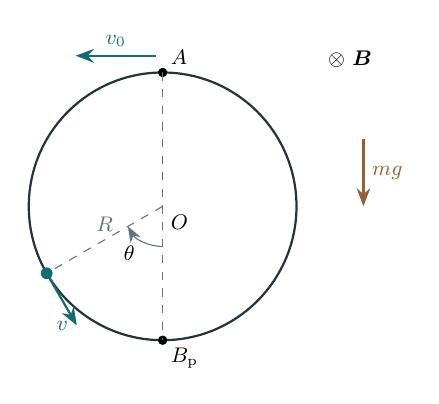
\begin{tikzpicture}[scale=.85,transform shape]

\draw[object] (0,0) circle (2);
\fill (0,2) circle (2pt) node[above right] {$A$};
\fill (0,-2) circle (2pt) node[below right] {$B_{\rm p}$};
\node[below right] at (0,0) {$O$};
\draw[guide] (0,2)--(0,-2);
\draw[motion] (-.1,2.25)--(-1.3,2.25) node[midway,above] {$v_0$};
\draw[guide] (0,0)--(-1.732,-1) node[midway,above] {$R$};
\fill[color=accent] (-1.732,-1) circle (2.5pt);
\draw[motion] (-1.732,-1)--(-1.282,-1.78) node[left] {$v$};
\draw[axis] (0,-.6) arc[start angle=-90,end angle=-150,radius=.6];
\node at (-.5,-.7) {$\theta$};
\draw[force] (3,1)--(3,0) node[midway,right] {$mg$};
\node at (2.8,2.2) {$\otimes\ \boldsymbol B$};

\end{tikzpicture}
\figcaption{图电试2.3\quad 质点沿左半环下降，磁力向心，圆环支持力向外。}
\end{minipage}\end{center}

\Needspace{6\baselineskip}\subsection*{解答}


图电试2.3中质点先沿左半环下降，磁力始终指向圆心，圆环支持力沿径向向外。设$\theta$为质点半径与竖直向下方向的夹角：$A$处$\theta=\pi$，$B_{\rm p}$处$\theta=0$，左半环上$\theta$随时间减小。

沿左半环可取位置$\boldsymbol r=(-R\sin\theta,-R\cos\theta)$，速度为$\boldsymbol v=(v\cos\theta,-v\sin\theta)$，其中$\dot\theta=-v/R$。磁场是$-B\hat z$，叉积$Q\boldsymbol v\times(-B\hat z)=QBv(\sin\theta,\cos\theta)$恰与位置矢量反向。最高点速度向左、最低点向右，磁力方向随切向速度连续转动，始终指向圆心。磁力和支持力都不做功，机械能守恒给
\[
\frac12mv^2=\frac12mv_0^2+mgR(1+\cos\theta),
\qquad
\boxed{\frac{v^2}{Rg}=\lambda+2+2\cos\theta}.
\]
最低点速度为$v_b=\sqrt{(\lambda+4)Rg}$。在最低点，磁力向上、重力和支持力向下，由向心方程
\[
\frac{mv_b^2}{R}=QBv_b-mg-N_b.
\]
最低点处向心方向向上。磁力提供向上的$QBv_b$，重力和外侧支持力都向下，故它们从可用向心合力中减去。$N_b$逐渐减到零时是本问指定的临界情况。第（1）问要求$N_b=0$，所以
\[
\lambda+4=\sqrt{\mu(\lambda+4)}-1,\qquad
\boxed{\mu=\frac{(\lambda+5)^2}{\lambda+4}}.
\]
质点下降时增加的动能全部来自重力势能的减少，磁力改变向心力的分配。
\begin{center}\begin{minipage}{.98\linewidth}\centering
\begin{tikzpicture}[scale=.68,transform shape]

\node at (0,2) {最高点 $A$};
\fill (0,0) circle (2.5pt);
\draw[force] (0,0)--(0,-1.2) node[right] {$QBv_0$};
\draw[force] (-.4,0)--(-.4,-.8) node[left] {$mg$};
\draw[force] (0,.2)--(0,1.2) node[right] {$N_A$};
\begin{scope}[xshift=4.5cm]
\node at (0,2) {一般位置};
\fill (0,0) circle (2.5pt);
\draw[guide] (-1.4,-.81)--(1.4,.81);
\draw[force] (0,0)--(1.04,.6) node[above right] {$QBv$};
\draw[force] (0,0)--(-1.04,-.6) node[below left] {$N$};
\draw[force] (0,-.1)--(0,-1.5) node[right] {$mg$};
\node at (0,-2.2) {向外：$mg\cos\theta-QBv+N$};
\end{scope}
\begin{scope}[xshift=9cm]
\node at (0,2) {最低点 $B_{\rm p}$};
\fill (0,0) circle (2.5pt);
\draw[force] (0,.1)--(0,1.25) node[right] {$QBv_b$};
\draw[force] (0,0)--(0,-1) node[right] {$mg$};
\node at (0,-1.7) {临界 $N_b=0$};
\end{scope}

\end{tikzpicture}
\figcaption{解图电试2.3A\quad 最高和最低位置的重力径向分量换号，磁力均向心。}
\end{minipage}\end{center}
解图电试2.3A分别画出最高、一般、最低位置的径向分量。取一般位置的径向向外为正，重力的向外分量为$mg\cos\theta$，磁力为$-QBv$，故
\[
-\frac{mv^2}{R}=mg\cos\theta-QBv+N.
\]
在一般点，$mg\cos\theta$在下半环向外、上半环向内；切向重力分量决定速率随位置怎样变化，径向重力分量则进入支持力方程。把能量得到的$v^2/(Rg)$和磁参数$QB/m=\sqrt{\mu g/R}$代入，磁力项化为$QBv/(mg)=\sqrt{\mu(\lambda+2+2\cos\theta)}$。于是令$c=\cos\theta$，
\[
\boxed{\frac N{mg}=n(c)
=\sqrt{\mu(\lambda+2+2c)}-(\lambda+2+3c)},
\qquad -1\le c\le1.
\]
最高点
\[
\frac{N_A}{mg}=\sqrt{\mu\lambda}-\lambda+1.
\]
若$0<\lambda\le1$，此式直接为正。若$\lambda>1$，需比较$\mu\lambda$与$(\lambda-1)^2$；代入临界关系，
\[
\mu\lambda-(\lambda-1)^2
=\frac{4(2\lambda^2+8\lambda-1)}{\lambda+4}>0.
\]
前一种情形中$1-\lambda\ge0$，再加正的磁项即为正。后一种情形只有在右侧$\lambda-1>0$时比较平方，代数差的分母$\lambda+4$为正，分子在$\lambda>1$也为正。因此第（2）问对所有$\lambda>0$均有$N_A>0$。

第（3）问还要把端点的正支持力条件延伸到全部中间位置。由
\[
n''(c)=-\frac{\sqrt\mu}{(\lambda+2+2c)^{3/2}}<0
\]
求导时$\lambda+2+2c\ge\lambda>0$，根号在整个闭区间内光滑，故二阶导数对每个位置都定义。可知$n$是凹函数，其图像位于连接两端点的弦线上方。临界关系下$n(1)=0$、$n(-1)>0$，故对$-1<c<1$，
\[
n(c)\ge\frac{1-c}{2}n(-1)>0.
\]
\begin{center}\begin{minipage}{.98\linewidth}\centering
\begin{tikzpicture}[scale=.8,transform shape]
\draw[axis] (0,0)--(10.7,0) node[right] {$c=\cos\theta$};
\draw[axis] (0,0)--(0,3.2) node[above] {$N/(mg)$};
\node[above] at (5,3.5) {$\lambda=1$：实线支持力，虚线端点弦线};
\draw[traj] plot coordinates {(0.000000000,2.683281573) (0.062500000,2.679115541) (0.125000000,2.674545417) (0.187500000,2.669585549) (0.250000000,2.664249456) (0.312500000,2.658549894) (0.375000000,2.652498914) (0.437500000,2.646107914) (0.500000000,2.639387691) (0.562500000,2.632348481) (0.625000000,2.625000000) (0.687500000,2.617351482) (0.750000000,2.609411708) (0.812500000,2.601189042) (0.875000000,2.592691454) (0.937500000,2.583926545) (1.000000000,2.574901573) (1.062500000,2.565623476) (1.125000000,2.556098884) (1.187500000,2.546334147) (1.250000000,2.536335345) (1.312500000,2.526108305) (1.375000000,2.515658618) (1.437500000,2.504991648) (1.500000000,2.494112550) (1.562500000,2.483026275) (1.625000000,2.471737588) (1.687500000,2.460251071) (1.750000000,2.448571137) (1.812500000,2.436702037) (1.875000000,2.424647870) (1.937500000,2.412412586) (2.000000000,2.400000000) (2.062500000,2.387413792) (2.125000000,2.374657518) (2.187500000,2.361734614) (2.250000000,2.348648402) (2.312500000,2.335402094) (2.375000000,2.321998799) (2.437500000,2.308441527) (2.500000000,2.294733192) (2.562500000,2.280876618) (2.625000000,2.266874542) (2.687500000,2.252729618) (2.750000000,2.238444419) (2.812500000,2.224021443) (2.875000000,2.209463115) (2.937500000,2.194771787) (3.000000000,2.179949748) (3.062500000,2.164999219) (3.125000000,2.149922359) (3.187500000,2.134721269) (3.250000000,2.119397990) (3.312500000,2.103954509) (3.375000000,2.088392760) (3.437500000,2.072714626) (3.500000000,2.056921938) (3.562500000,2.041016483) (3.625000000,2.025000000) (3.687500000,2.008874184) (3.750000000,1.992640687) (3.812500000,1.976301121) (3.875000000,1.959857057) (3.937500000,1.943310028) (4.000000000,1.926661531) (4.062500000,1.909913024) (4.125000000,1.893065934) (4.187500000,1.876121651) (4.250000000,1.859081537) (4.312500000,1.841946918) (4.375000000,1.824719092) (4.437500000,1.807399328) (4.500000000,1.789988864) (4.562500000,1.772488914) (4.625000000,1.754900661) (4.687500000,1.737225266) (4.750000000,1.719463864) (4.812500000,1.701617562) (4.875000000,1.683687449) (4.937500000,1.665674586) (5.000000000,1.647580015) (5.062500000,1.629404756) (5.125000000,1.611149806) (5.187500000,1.592816142) (5.250000000,1.574404724) (5.312500000,1.555916490) (5.375000000,1.537352360) (5.437500000,1.518713235) (5.500000000,1.500000000) (5.562500000,1.481213521) (5.625000000,1.462354649) (5.687500000,1.443424217) (5.750000000,1.424423043) (5.812500000,1.405351929) (5.875000000,1.386211663) (5.937500000,1.367003018) (6.000000000,1.347726751) (6.062500000,1.328383607) (6.125000000,1.308974318) (6.187500000,1.289499600) (6.250000000,1.269960159) (6.312500000,1.250356687) (6.375000000,1.230689864) (6.437500000,1.210960358) (6.500000000,1.191168825) (6.562500000,1.171315910) (6.625000000,1.151402247) (6.687500000,1.131428460) (6.750000000,1.111395160) (6.812500000,1.091302950) (6.875000000,1.071152423) (6.937500000,1.050944159) (7.000000000,1.030678732) (7.062500000,1.010356705) (7.125000000,0.989978632) (7.187500000,0.969545058) (7.250000000,0.949056520) (7.312500000,0.928513544) (7.375000000,0.907916650) (7.437500000,0.887266350) (7.500000000,0.866563146) (7.562500000,0.845807533) (7.625000000,0.825000000) (7.687500000,0.804141026) (7.750000000,0.783231083) (7.812500000,0.762270637) (7.875000000,0.741260147) (7.937500000,0.720200065) (8.000000000,0.699090834) (8.062500000,0.677932893) (8.125000000,0.656726674) (8.187500000,0.635472603) (8.250000000,0.614171097) (8.312500000,0.592822571) (8.375000000,0.571427432) (8.437500000,0.549986080) (8.500000000,0.528498912) (8.562500000,0.506966317) (8.625000000,0.485388679) (8.687500000,0.463766379) (8.750000000,0.442099788) (8.812500000,0.420389277) (8.875000000,0.398635209) (8.937500000,0.376837941) (9.000000000,0.354997828) (9.062500000,0.333115219) (9.125000000,0.311190457) (9.187500000,0.289223882) (9.250000000,0.267215829) (9.312500000,0.245166629) (9.375000000,0.223076607) (9.437500000,0.200946086) (9.500000000,0.178775383) (9.562500000,0.156564811) (9.625000000,0.134314681) (9.687500000,0.112025297) (9.750000000,0.089696962) (9.812500000,0.067329972) (9.875000000,0.044924623) (9.937500000,0.022481203) (10.000000000,0.000000000)};
\draw[dashed,thick,color=warm] plot coordinates {(0.000000000,2.683281573) (0.062500000,2.666511063) (0.125000000,2.649740553) (0.187500000,2.632970044) (0.250000000,2.616199534) (0.312500000,2.599429024) (0.375000000,2.582658514) (0.437500000,2.565888004) (0.500000000,2.549117494) (0.562500000,2.532346985) (0.625000000,2.515576475) (0.687500000,2.498805965) (0.750000000,2.482035455) (0.812500000,2.465264945) (0.875000000,2.448494435) (0.937500000,2.431723926) (1.000000000,2.414953416) (1.062500000,2.398182906) (1.125000000,2.381412396) (1.187500000,2.364641886) (1.250000000,2.347871376) (1.312500000,2.331100867) (1.375000000,2.314330357) (1.437500000,2.297559847) (1.500000000,2.280789337) (1.562500000,2.264018827) (1.625000000,2.247248317) (1.687500000,2.230477808) (1.750000000,2.213707298) (1.812500000,2.196936788) (1.875000000,2.180166278) (1.937500000,2.163395768) (2.000000000,2.146625258) (2.062500000,2.129854749) (2.125000000,2.113084239) (2.187500000,2.096313729) (2.250000000,2.079543219) (2.312500000,2.062772709) (2.375000000,2.046002199) (2.437500000,2.029231690) (2.500000000,2.012461180) (2.562500000,1.995690670) (2.625000000,1.978920160) (2.687500000,1.962149650) (2.750000000,1.945379140) (2.812500000,1.928608631) (2.875000000,1.911838121) (2.937500000,1.895067611) (3.000000000,1.878297101) (3.062500000,1.861526591) (3.125000000,1.844756081) (3.187500000,1.827985572) (3.250000000,1.811215062) (3.312500000,1.794444552) (3.375000000,1.777674042) (3.437500000,1.760903532) (3.500000000,1.744133022) (3.562500000,1.727362513) (3.625000000,1.710592003) (3.687500000,1.693821493) (3.750000000,1.677050983) (3.812500000,1.660280473) (3.875000000,1.643509963) (3.937500000,1.626739454) (4.000000000,1.609968944) (4.062500000,1.593198434) (4.125000000,1.576427924) (4.187500000,1.559657414) (4.250000000,1.542886904) (4.312500000,1.526116395) (4.375000000,1.509345885) (4.437500000,1.492575375) (4.500000000,1.475804865) (4.562500000,1.459034355) (4.625000000,1.442263845) (4.687500000,1.425493336) (4.750000000,1.408722826) (4.812500000,1.391952316) (4.875000000,1.375181806) (4.937500000,1.358411296) (5.000000000,1.341640786) (5.062500000,1.324870277) (5.125000000,1.308099767) (5.187500000,1.291329257) (5.250000000,1.274558747) (5.312500000,1.257788237) (5.375000000,1.241017728) (5.437500000,1.224247218) (5.500000000,1.207476708) (5.562500000,1.190706198) (5.625000000,1.173935688) (5.687500000,1.157165178) (5.750000000,1.140394669) (5.812500000,1.123624159) (5.875000000,1.106853649) (5.937500000,1.090083139) (6.000000000,1.073312629) (6.062500000,1.056542119) (6.125000000,1.039771610) (6.187500000,1.023001100) (6.250000000,1.006230590) (6.312500000,0.989460080) (6.375000000,0.972689570) (6.437500000,0.955919060) (6.500000000,0.939148551) (6.562500000,0.922378041) (6.625000000,0.905607531) (6.687500000,0.888837021) (6.750000000,0.872066511) (6.812500000,0.855296001) (6.875000000,0.838525492) (6.937500000,0.821754982) (7.000000000,0.804984472) (7.062500000,0.788213962) (7.125000000,0.771443452) (7.187500000,0.754672942) (7.250000000,0.737902433) (7.312500000,0.721131923) (7.375000000,0.704361413) (7.437500000,0.687590903) (7.500000000,0.670820393) (7.562500000,0.654049883) (7.625000000,0.637279374) (7.687500000,0.620508864) (7.750000000,0.603738354) (7.812500000,0.586967844) (7.875000000,0.570197334) (7.937500000,0.553426824) (8.000000000,0.536656315) (8.062500000,0.519885805) (8.125000000,0.503115295) (8.187500000,0.486344785) (8.250000000,0.469574275) (8.312500000,0.452803765) (8.375000000,0.436033256) (8.437500000,0.419262746) (8.500000000,0.402492236) (8.562500000,0.385721726) (8.625000000,0.368951216) (8.687500000,0.352180706) (8.750000000,0.335410197) (8.812500000,0.318639687) (8.875000000,0.301869177) (8.937500000,0.285098667) (9.000000000,0.268328157) (9.062500000,0.251557647) (9.125000000,0.234787138) (9.187500000,0.218016628) (9.250000000,0.201246118) (9.312500000,0.184475608) (9.375000000,0.167705098) (9.437500000,0.150934588) (9.500000000,0.134164079) (9.562500000,0.117393569) (9.625000000,0.100623059) (9.687500000,0.083852549) (9.750000000,0.067082039) (9.812500000,0.050311529) (9.875000000,0.033541020) (9.937500000,0.016770510) (10.000000000,0.000000000)};
\node[below] at (0,-.12) {$-1$};
\node[below] at (5,-.12) {$0$};
\node[below] at (10,-.12) {$1$};
\end{tikzpicture}
\figcaption{解图电试2.3B\quad $\lambda=1$：实线支持力，虚线端点弦线}
\end{minipage}\end{center}
弦线在$c=-1$取$n(-1)$，在$c=1$取0，其内点值为$(1-c)n(-1)/2$。因为内点$c<1$且$n(-1)>0$，整条弦线在内部为正；凹函数又在弦线上方，正支持力因而覆盖每个中间角度。这一步把端点条件与连续轨迹之间的关系明确写出。

解图电试2.3B中的曲线只在最低点$c=1$与零轴相接；最高点及全部中间位置均为正。故所求全部范围为
\[
\boxed{\lambda>0}.
\]
平方方法进一步说明含平方根不等式的符号条件。若$\lambda+2+3c\le0$，正的平方根已使$n(c)>0$。若$\lambda+2+3c>0$，比较两边平方，差的分子为
\[
\begin{aligned}
D(c)&=(\lambda+5)^2(\lambda+2+2c)
-(\lambda+4)(\lambda+2+3c)^2\\
&=(1-c)\bigl[9(\lambda+4)c+(\lambda+2)(4\lambda+17)\bigr].
\end{aligned}
\]
因式$1-c$在中间位置为正，判断平方差便归结到方括号的符号。它是$c$的一次函数，系数$9(\lambda+4)>0$，因此取允许区间的最小$c$即可得到下界。当$\lambda\ge1$时，方括号在$c>-1$范围的下界为
$2(2\lambda^2+8\lambda-1)>0$。当$0<\lambda<1$时，可平方的前提要求$c>-(\lambda+2)/3$，方括号因而大于
$(\lambda+2)(\lambda+5)>0$。在上述两个符号区间内，全部中间位置都得到$N>0$。

第（4）问右半环速度沿环向上，但磁力仍向圆心，同一$N(c)$公式继续适用。回到$A$时恢复初速，之后重复运动。最低点只有孤立的$N=0$，两侧支持力均为正，质点可以保持接触并通过该点：
\[
n(\cos\theta)
=\frac{2\lambda+7}{2(\lambda+4)}\theta^2+O(\theta^4)
\quad(\theta\to0).
\]
\begin{center}\begin{minipage}{.98\linewidth}\centering
\begin{tikzpicture}[scale=.8,transform shape]
\draw[axis] (0,0)--(10.7,0) node[right] {$\theta$};
\draw[axis] (0,0)--(0,3.2) node[above] {$N/(mg)$};\foreach \y/\lab in {0/0,1/0.05,2/0.1}{\draw[thin] (0,\y)--(-.08,\y) node[left] {$\lab$};}
\node[above] at (5,3.5) {最低点附近的正支持力与二次主项};
\draw[traj] plot coordinates {(0.000000000,2.826608060) (0.083333333,2.734868162) (0.166666667,2.644557845) (0.250000000,2.555682743) (0.333333333,2.468248401) (0.416666667,2.382260273) (0.500000000,2.297723724) (0.583333333,2.214644026) (0.666666667,2.133026361) (0.750000000,2.052875818) (0.833333333,1.974197396) (0.916666667,1.896996000) (1.000000000,1.821276443) (1.083333333,1.747043447) (1.166666667,1.674301638) (1.250000000,1.603055552) (1.333333333,1.533309628) (1.416666667,1.465068213) (1.500000000,1.398335561) (1.583333333,1.333115829) (1.666666667,1.269413081) (1.750000000,1.207231288) (1.833333333,1.146574322) (1.916666667,1.087445963) (2.000000000,1.029849893) (2.083333333,0.973789702) (2.166666667,0.919268880) (2.250000000,0.866290823) (2.333333333,0.814858831) (2.416666667,0.764976107) (2.500000000,0.716645758) (2.583333333,0.669870792) (2.666666667,0.624654122) (2.750000000,0.580998564) (2.833333333,0.538906836) (2.916666667,0.498381558) (3.000000000,0.459425254) (3.083333333,0.422040347) (3.166666667,0.386229167) (3.250000000,0.351993942) (3.333333333,0.319336802) (3.416666667,0.288259781) (3.500000000,0.258764813) (3.583333333,0.230853733) (3.666666667,0.204528280) (3.750000000,0.179790090) (3.833333333,0.156640704) (3.916666667,0.135081563) (4.000000000,0.115114008) (4.083333333,0.096739281) (4.166666667,0.079958526) (4.250000000,0.064772788) (4.333333333,0.051183011) (4.416666667,0.039190041) (4.500000000,0.028794624) (4.583333333,0.019997408) (4.666666667,0.012798938) (4.750000000,0.007199664) (4.833333333,0.003199934) (4.916666667,0.000799996) (5.000000000,0.000000000) (5.083333333,0.000799996) (5.166666667,0.003199934) (5.250000000,0.007199664) (5.333333333,0.012798938) (5.416666667,0.019997408) (5.500000000,0.028794624) (5.583333333,0.039190041) (5.666666667,0.051183011) (5.750000000,0.064772788) (5.833333333,0.079958526) (5.916666667,0.096739281) (6.000000000,0.115114008) (6.083333333,0.135081563) (6.166666667,0.156640704) (6.250000000,0.179790090) (6.333333333,0.204528280) (6.416666667,0.230853733) (6.500000000,0.258764813) (6.583333333,0.288259781) (6.666666667,0.319336802) (6.750000000,0.351993942) (6.833333333,0.386229167) (6.916666667,0.422040347) (7.000000000,0.459425254) (7.083333333,0.498381558) (7.166666667,0.538906836) (7.250000000,0.580998564) (7.333333333,0.624654122) (7.416666667,0.669870792) (7.500000000,0.716645758) (7.583333333,0.764976107) (7.666666667,0.814858831) (7.750000000,0.866290823) (7.833333333,0.919268880) (7.916666667,0.973789702) (8.000000000,1.029849893) (8.083333333,1.087445963) (8.166666667,1.146574322) (8.250000000,1.207231288) (8.333333333,1.269413081) (8.416666667,1.333115829) (8.500000000,1.398335561) (8.583333333,1.465068213) (8.666666667,1.533309628) (8.750000000,1.603055552) (8.833333333,1.674301638) (8.916666667,1.747043447) (9.000000000,1.821276443) (9.083333333,1.896996000) (9.166666667,1.974197396) (9.250000000,2.052875818) (9.333333333,2.133026361) (9.416666667,2.214644026) (9.500000000,2.297723724) (9.583333333,2.382260273) (9.666666667,2.468248401) (9.750000000,2.555682743) (9.833333333,2.644557845) (9.916666667,2.734868162) (10.000000000,2.826608060)};
\draw[dashed,thick,color=warm] plot coordinates {(0.000000000,2.880000000) (0.083333333,2.784800000) (0.166666667,2.691200000) (0.250000000,2.599200000) (0.333333333,2.508800000) (0.416666667,2.420000000) (0.500000000,2.332800000) (0.583333333,2.247200000) (0.666666667,2.163200000) (0.750000000,2.080800000) (0.833333333,2.000000000) (0.916666667,1.920800000) (1.000000000,1.843200000) (1.083333333,1.767200000) (1.166666667,1.692800000) (1.250000000,1.620000000) (1.333333333,1.548800000) (1.416666667,1.479200000) (1.500000000,1.411200000) (1.583333333,1.344800000) (1.666666667,1.280000000) (1.750000000,1.216800000) (1.833333333,1.155200000) (1.916666667,1.095200000) (2.000000000,1.036800000) (2.083333333,0.980000000) (2.166666667,0.924800000) (2.250000000,0.871200000) (2.333333333,0.819200000) (2.416666667,0.768800000) (2.500000000,0.720000000) (2.583333333,0.672800000) (2.666666667,0.627200000) (2.750000000,0.583200000) (2.833333333,0.540800000) (2.916666667,0.500000000) (3.000000000,0.460800000) (3.083333333,0.423200000) (3.166666667,0.387200000) (3.250000000,0.352800000) (3.333333333,0.320000000) (3.416666667,0.288800000) (3.500000000,0.259200000) (3.583333333,0.231200000) (3.666666667,0.204800000) (3.750000000,0.180000000) (3.833333333,0.156800000) (3.916666667,0.135200000) (4.000000000,0.115200000) (4.083333333,0.096800000) (4.166666667,0.080000000) (4.250000000,0.064800000) (4.333333333,0.051200000) (4.416666667,0.039200000) (4.500000000,0.028800000) (4.583333333,0.020000000) (4.666666667,0.012800000) (4.750000000,0.007200000) (4.833333333,0.003200000) (4.916666667,0.000800000) (5.000000000,0.000000000) (5.083333333,0.000800000) (5.166666667,0.003200000) (5.250000000,0.007200000) (5.333333333,0.012800000) (5.416666667,0.020000000) (5.500000000,0.028800000) (5.583333333,0.039200000) (5.666666667,0.051200000) (5.750000000,0.064800000) (5.833333333,0.080000000) (5.916666667,0.096800000) (6.000000000,0.115200000) (6.083333333,0.135200000) (6.166666667,0.156800000) (6.250000000,0.180000000) (6.333333333,0.204800000) (6.416666667,0.231200000) (6.500000000,0.259200000) (6.583333333,0.288800000) (6.666666667,0.320000000) (6.750000000,0.352800000) (6.833333333,0.387200000) (6.916666667,0.423200000) (7.000000000,0.460800000) (7.083333333,0.500000000) (7.166666667,0.540800000) (7.250000000,0.583200000) (7.333333333,0.627200000) (7.416666667,0.672800000) (7.500000000,0.720000000) (7.583333333,0.768800000) (7.666666667,0.819200000) (7.750000000,0.871200000) (7.833333333,0.924800000) (7.916666667,0.980000000) (8.000000000,1.036800000) (8.083333333,1.095200000) (8.166666667,1.155200000) (8.250000000,1.216800000) (8.333333333,1.280000000) (8.416666667,1.344800000) (8.500000000,1.411200000) (8.583333333,1.479200000) (8.666666667,1.548800000) (8.750000000,1.620000000) (8.833333333,1.692800000) (8.916666667,1.767200000) (9.000000000,1.843200000) (9.083333333,1.920800000) (9.166666667,2.000000000) (9.250000000,2.080800000) (9.333333333,2.163200000) (9.416666667,2.247200000) (9.500000000,2.332800000) (9.583333333,2.420000000) (9.666666667,2.508800000) (9.750000000,2.599200000) (9.833333333,2.691200000) (9.916666667,2.784800000) (10.000000000,2.880000000)};
\node[below] at (0,-.12) {$-0.4$};
\node[below] at (5,-.12) {$0$};
\node[below] at (10,-.12) {$0.4$};
\end{tikzpicture}
\figcaption{解图电试2.3C\quad 最低点附近的正支持力与二次主项}
\end{minipage}\end{center}
图C把最低点左右两侧的小角画在同一坐标中，实线为完整支持力，虚线为二次主项。质点通过时$v_b>0$，位置和速度连续；支持力连续降到零再升起，其所需方向始终沿外法线，因此圆环可维持这一约束运动。取连续角从$\pi$经0减到$-\pi$，同一个位置公式覆盖右半环，叉积的向心磁力关系也继续成立。

一般$\mu$下，凹性说明全环的最小支持力出现在两个端点之一。最低点条件为
$\mu\ge(\lambda+5)^2/(\lambda+4)$；最高点在$\lambda\le1$时自动满足，$\lambda>1$时要求$\mu\ge(\lambda-1)^2/\lambda$，后者弱于最低点条件。当$\lambda>1$，两端场强阈值之差为$4(2\lambda^2+8\lambda-1)/[\lambda(\lambda+4)]>0$，所以最低点给出的要求较强；当$\lambda\le1$时最高点本已满足非负支持力。又因$n(c)$为凹函数，满足这两个端点条件就覆盖整个圆环。因此
\[
\boxed{\lambda>0,\qquad
\mu\ge\frac{(\lambda+5)^2}{\lambda+4}}
\]
是这一方向持续绕行的条件；若要求全环处处严格$N>0$，将第二个不等号改成$>$。$\lambda=0$对应最高点严格静止的初态，切向力恰为零，质点停留在这个平衡位置；$\lambda\to0^+$则始终保留非零初速，绕行所需时间随初速减小而增加。
磁场提供向内偏转，沿环速率由能量式确定。临界磁场下，重力在下降半环增加动能，在上升半环取回相同动能，质点回到最高点时速度大小、方向和机械能都恢复；均匀静磁场、固定光滑环和无阻力条件于是使下一周重复同一过程。接触期间的绕行时间由$\mathrm dt=R|\mathrm d\theta|/v$积分，初速很小时主要时间花在最高点附近，实际运动与严格静止初态因此有不同的时间行为。



\Needspace{13\baselineskip}

\pdfbookmark[2]{第 4 题 匀强磁场中电阻网络的总安培力}{q4}

\section*{第 4 题\quad 匀强磁场中电阻网络的总安培力}\label{q:4}


平面$\Sigma_1$与$\Sigma_2$相交于直线$MN$，夹角$\phi=45^\circ$。匀强磁场$\boldsymbol B$平行于$\Sigma_1$、垂直$MN$。
$\Sigma_2$内有长方形网络$abcdef$：$a,b$为左下、左上角，$d,e$为右上、右下角，$c,f$分别是上下长边中点。七段$ab,bc,cd,de,ef,fa,fc$均长$l$，且$ab\parallel MN$。各电阻为
\[
R_{ab}=R_{fc}=R_{ed}=R,\quad
R_{af}=R_{bc}=2R,\quad R_{fe}=R_{cd}=4R.
\]
总电流$I$从$a$流入、从$d$流出。求网络所受总磁场力大小，并说明是否需要先求七段电流。
取$\hat e_u$由$a$指向$f$，$\hat e_v$由$a$指向$b$，$\hat n=\hat e_u\times\hat e_v$，选择磁场为
$\boldsymbol B=B(\cos\phi\,\hat e_u+\sin\phi\,\hat n)$。


\begin{center}\begin{minipage}{.98\linewidth}\centering
\begin{tikzpicture}[scale=.7,transform shape]

\coordinate (a) at (0,0);\coordinate (b) at (0,2);
\coordinate (c) at (2,2);\coordinate (d) at (4,2);
\coordinate (e) at (4,0);\coordinate (f) at (2,0);
\foreach \p/\q/\lab in {a/b/R,b/c/2R,c/d/4R,d/e/R,e/f/4R,f/a/2R,f/c/R}{
\draw[object] (\p)--(\q) node[midway,fill=white,inner sep=2pt] {$\lab$};}
\foreach \p in {a,b,c,d,e,f}{\fill (\p) circle (1.6pt);}
\node[below left] at (a) {$a$};\node[above left] at (b) {$b$};
\node[above] at (c) {$c$};\node[above right] at (d) {$d$};
\node[below right] at (e) {$e$};\node[below] at (f) {$f$};
\draw[motion] (-1,0)--(-.15,0) node[midway,above] {$I$};
\draw[motion] (4.15,2)--(5,2) node[midway,above] {$I$};
\draw[axis] (-.7,-.7)--(1,-.7) node[right] {$\hat e_u$};
\draw[axis] (-.7,-.7)--(-.7,1) node[left] {$\hat e_v\parallel MN$};

\begin{scope}[xshift=8cm,yshift=.3cm]
\draw[axis] (0,0)--(2.7,0) node[right] {$\Sigma_2,\hat e_u$};
\draw[axis] (0,0)--(0,2.6) node[above] {$\hat n$};
\draw[motion] (0,0)--(1.8,1.8) node[right] {$\boldsymbol B$};
\draw[guide] (-.5,-.5)--(2.1,2.1) node[above] {$\Sigma_1$};
\draw[axis] (.7,0) arc[start angle=0,end angle=45,radius=.7];
\node at (1,.42) {$\phi$};
\node[align=center] at (1.2,-1) {沿$MN$观察\\截面};
\end{scope}

\end{tikzpicture}
\figcaption{图电试2.4\quad 网络长边为两段l；右侧截面给磁场与网络面的夹角。}
\end{minipage}\end{center}

\Needspace{6\baselineskip}\subsection*{解答}


图电试2.4中各段电流大小会随电阻改变，但任一内部结点都满足电流守恒。先以任意有向线段$i\to j$表示一个支路，电流代数值为$I_{ij}$。匀强场中该段磁场力为
\[
\boldsymbol F_{ij}
=I_{ij}(\boldsymbol r_j-\boldsymbol r_i)\times\boldsymbol B.
\]
匀强磁场在每个支路上取同一个矢量，所以先把电流乘位移求和，再与$\boldsymbol B$作叉积。对结点$k$，每条流入支路给$+I\boldsymbol r_k$，每条流出支路给$-I\boldsymbol r_k$。把网络全部支路相加。每个内部结点的$\boldsymbol r_k$系数等于流入电流减流出电流，因结点守恒而为零；只剩输入、输出结点：
\[
\sum I_{ij}(\boldsymbol r_j-\boldsymbol r_i)
=I(\boldsymbol r_d-\boldsymbol r_a).
\]
\begin{center}\begin{minipage}{.98\linewidth}\centering
\begin{tikzpicture}[scale=.8,transform shape]

\draw[object] (0,0) rectangle (4,2);
\draw[guide] (2,0)--(2,2);
\node[below left] at (0,0) {$a$};\node[above right] at (4,2) {$d$};
\draw[motion] (.1,.05)--(1.2,.6);
\draw[motion] (1.5,.75)--(3.8,1.9);
\node[above,rotate=26.565] at (2,1.2) {$I(\boldsymbol r_d-\boldsymbol r_a)$};
\node at (0,2.8) {端点保留};
\begin{scope}[xshift=6.5cm]
\draw[object] (0,0) rectangle (2,2);
\draw[motion] (.3,0)--(1.5,0);
\draw[motion] (2,.3)--(2,1.5);
\draw[motion] (1.7,2)--(.5,2);
\draw[motion] (0,1.7)--(0,.5);
\node at (1,2.8) {内部闭合电流};
\node at (1,-.9) {$\oint d\boldsymbol l=0$};
\end{scope}
\node at (3.8,-1.6) {结点守恒使内部位置矢量的系数相消};

\end{tikzpicture}
\figcaption{解图电试2.4A\quad 网络可叠加为开路径与闭合回路，闭合部分在匀强场中合力为零。}
\end{minipage}\end{center}
解图电试2.4A用闭合小回路与从$a$到$d$的开路径分解同一网络。任一闭合回路满足$\oint d\boldsymbol l=0$，故在匀强场中合力为零。于是整个网络与一段从$a$指向$d$、电流为$I$的假想直导线具有相同合力：
\[
\boxed{\boldsymbol F
=I(\boldsymbol r_d-\boldsymbol r_a)\times\boldsymbol B}.
\]
所取受力对象是题图的网络部分；电源回线与引线作为另一部分单独计算磁场力。

图A的分解也可写为沿上边的$a\to b\to c\to d$路径、沿下边的$a\to f\to e\to d$路径与右侧方环$f\to c\to d\to e\to f$。两条开放路径分别以各自电流连接相同端点，电流之和为$I$；叠加方环的每个支路变化在结点处相互抵消，环的位移和为零。于是无论怎样分流，求合力都保留同一端点向量。

图中位移为
\[
\boldsymbol r_d-\boldsymbol r_a=2l\hat e_u+l\hat e_v.
\]
几何上$ad$由两段水平长度$l$与一段高度$l$组成，长度为$\sqrt{(2l)^2+l^2}=\sqrt5l$。基底满足$\hat e_u\times\hat e_v=\hat n$、$\hat e_v\times\hat n=\hat e_u$、$\hat n\times\hat e_u=\hat e_v$，交换叉积次序则变号。用$\hat e_u\times\hat e_v=\hat n$逐项作叉积，
\[
\boldsymbol F
=IBl\bigl(\sin\phi\,\hat e_u
-2\sin\phi\,\hat e_v-\cos\phi\,\hat n\bigr).
\]
\begin{center}\begin{minipage}{.98\linewidth}\centering
\begin{tikzpicture}[scale=.85,transform shape]

\coordinate (A) at (0,0);\coordinate (P) at (2.12132,0);\coordinate (D) at (2.12132,2.59808);
\draw[motion] (A)--(D) node[midway,above left] {$\boldsymbol r_d-\boldsymbol r_a$};
\draw[guide] (A)--(P) node[midway,below] {$2l\cos\phi$};
\draw[force] (P)--(D) node[midway,right] {$L_\perp$};
\draw[object] (1.87132,0)--(1.87132,.25)--(2.12132,.25);
\draw[axis] (-.5,0)--(4.5,0) node[right] {$\boldsymbol B$方向};
\node[below left] at (A) {$a$};\node[above right] at (D) {$d$};
\node at (1.7,3.4) {$|ad|=\sqrt5l,\quad\phi=45^\circ$};
\node at (2,-1.2) {$L_\perp=\sqrt{5l^2-4l^2\cos^2\phi}=\sqrt3l$};

\end{tikzpicture}
\figcaption{解图电试2.4B\quad 从端点位移中去掉平行磁场的投影，余下长度决定总力大小。}
\end{minipage}\end{center}
解图电试2.4B将位移投影到沿$\boldsymbol B$和垂直$\boldsymbol B$的方向。端点距离$|ad|=\sqrt5l$包含沿场分量和垂直场分量，所用有效长度取后者：其沿磁场投影为$2l\cos\phi$，所以
\[
L_\perp^2=|ad|^2-(2l\cos\phi)^2
=l^2(1+4\sin^2\phi).
\]
磁场沿$MN$方向的分量为零，因此$l\hat e_v$与磁场垂直；$2l\hat e_u$的沿场投影为$2l\cos\phi$。这与$ad$直接对单位磁场点积的结果相同。若把对角线与磁场夹角记作$\theta$，则$\cos\theta=2\cos\phi/\sqrt5$；在45度时$\sin\theta=\sqrt{3/5}$。因此
\[
F=IBl\sqrt{1+4\sin^2\phi},\qquad
\boxed{F=\sqrt3\,IBl\quad(\phi=45^\circ)}.
\]
这也与矢量表达式各正交分量的平方和相符。

\begin{center}\begin{minipage}{.98\linewidth}\centering
\begin{tikzpicture}[scale=.8,transform shape]
\draw[very thick] (0,0)--(0,2)--(2,2)--(4,2)--(4,0)--(2,0)--cycle;\draw[very thick] (2,0)--(2,2);\node[below left] at (0,0) {$a$};\node[above left] at (0,2) {$b$};\node[above] at (2,2) {$c$};\node[above right] at (4,2) {$d$};\node[below right] at (4,0) {$e$};\node[below] at (2,0) {$f$};\node[left] at (0,1) {$25$向上};\node[above] at (1,2) {$25\to$};\node[above] at (3,2) {$32\to$};\node[right] at (4,1) {$27$向上};\node[below] at (1,0) {$34\to$};\node[below] at (3,0) {$27\to$};\node[right] at (2,1) {$7$向上};\node at (2,-1.6) {各数值的电流单位为$I/59$};
\end{tikzpicture}
\figcaption{解图电试2.4C\quad 给定电阻网络中七个支路电流满足全部结点守恒}
\end{minipage}\end{center}
给定电阻数据可具体显示上述分流。令$V_d=0$，以$IR$为电势单位，先列输入点与三个普通结点的方程：
\[
\begin{aligned}
&(V_a-V_b)/R+(V_a-V_f)/(2R)=I,\\
&(V_b-V_a)/R+(V_b-V_c)/(2R)=0,\\
&(V_c-V_b)/(2R)+V_c/(4R)+(V_c-V_f)/R=0,\\
&V_e/R+(V_e-V_f)/(4R)=0.
\end{aligned}
\]
再与下面$f$点的方程联立，求五个非接地结点电势，得
\[
(V_a,V_b,V_c,V_e,V_f)
=\frac{IR}{59}(203,178,128,27,135).
\]
例如$f$结点满足
\[
\frac{V_f-V_a}{2R}
+\frac{V_f-V_e}{4R}
+\frac{V_f-V_c}{R}=0.
\]
对应各段电流为
\[
(I_{ab},I_{bc},I_{cd},I_{ed},I_{fe},I_{af},I_{fc})
=\frac I{59}(25,25,32,27,27,34,7),
\]
下标已指明方向。$a$处$25I/59+34I/59=I$，$d$处$32I/59+27I/59=I$，其余结点也守恒。将这些电流逐段乘位移相加，仍恰为$I(2l\hat e_u+l\hat e_v)$。所以固定总电流时，端点位移与电流守恒已经确定网络合力；若固定的是端电压，电阻会通过$I$影响合力。
这组电流可按图A具体分解：上方开放路径电流为$25I/59$，下方开放路径电流为$34I/59$，右方闭合环流为$7I/59$。所以$cd$电流为$(25+7)I/59$，$fe$与$ed$电流为$(34-7)I/59$，其余支路分别保持对应路径电流。两条开放路径各自的电流乘位移均沿$ad$，闭合环的四个位移相加为零，直接给总和$I(2l\hat e_u+l\hat e_v)$。结点法说明具体电流怎样分配，端点法说明这种分配为何从总力中消去；它们描述的是同一个稳恒网络。



\Needspace{13\baselineskip}

\pdfbookmark[2]{第 5 题 时变磁场中带电弦杆的转动与端点作用力}{q5}

\section*{第 5 题\quad 时变磁场中带电弦杆的转动与端点作用力}\label{q:5}


半径$R$的光滑绝缘圆环固定在水平面内。以环为横截面的竖直圆柱区域内有磁场
$\boldsymbol B=-B(t)\hat z$，其中$B(t)=B_0\sin\omega_0t$、$B_0>0$，$\hat z$竖直向上；柱外磁场为零。采用轴对称的感应电场，忽略附加静电场、自场和辐射。
均匀绝缘刚性细杆$ab$总质量$m$、总正电荷$Q$，其质心$C$距环心$O$为$D=R/2$，两端由光滑的双向径向约束保持在圆周上。电荷分布始终均匀；重力由水平支承平衡，只求水平面内作用力。
$t=0$时杆静止，此后先逆时针转过$2\pi$，再顺时针返回$2\pi$，如此交替。
\begin{enumerate}
\item 求$\omega_0$与$m,Q,B_0$的关系。
\item 求杆在$a,b$端对约束圆环的水平作用力随时间的变化，给出大小和实际方向。
\item 说明上述双向约束若改为只能向杆施加朝向$O$压力的普通单侧内壁，给定运动能否实现。
\end{enumerate}
令$\hat e_r$由$O$指向$C$，$\hat e_t=\hat z\times\hat e_r$；初始杆沿$\hat e_t$，$a$在$C$的负$\hat e_t$侧，$b$在正侧。


\begin{center}\begin{minipage}{.98\linewidth}\centering
\begin{tikzpicture}[scale=.75,transform shape]

\draw[object] (0,0) circle (2);
\draw[object,line width=1.5pt] (1,-1.732)--(1,1.732);
\fill (0,0) circle (1.5pt) node[below left] {$O$};
\fill[color=accent] (1,0) circle (2pt) node[below right] {$C$};
\node[below right] at (1,-1.732) {$a$};
\node[above right] at (1,1.732) {$b$};
\draw[guide] (0,0)--(1,0) node[midway,below] {$D$};
\draw[guide] (0,0)--(1,1.732) node[midway,above left] {$R$};

\draw[axis] (0,0)--(2.7,0) node[right] {$\hat e_r$};
\draw[axis] (1,.15)--(1,2.5) node[above] {$\hat e_t$};
\node at (-1,1) {$\otimes\ B(t)$};
\node at (0,-2.6) {$D=R/2,\quad L=\sqrt3D$};
\node[align=left] at (4.8,1) {杆：均匀$m,Q$\\初始静止\\端点双向径向约束};

\end{tikzpicture}
\figcaption{图电试2.5\quad 俯视水平圆环，a、b的标记随杆运动而保持。}
\end{minipage}\end{center}

\Needspace{6\baselineskip}\subsection*{解答}


图电试2.5中半杆长记为$L$，由弦的几何关系，
\[
D=\frac R2,\qquad L=\sqrt{R^2-D^2}=\sqrt3D.
\]
杆两端在同一圆周上，连接环心与弦中点的半径垂直杆，勾股关系给$D^2+L^2=R^2$。半杆长是$L$，完整杆长是$2L$，因此均匀质量与电荷的线密度分别为$m/(2L)$与$Q/(2L)$。随杆转动的基矢为$\hat e_r,\hat e_t$。用$s\in[-L,L]$标记杆上的电荷元，则相对于固定环心$O$，
\[
\boldsymbol r=D\hat e_r+s\hat e_t,\qquad
dq=\frac Q{2L}\,ds,\quad dm=\frac m{2L}\,ds.
\]
转角$\theta$取逆时针为正，$\Omega=\dot\theta$。整根杆绕固定$O$转动，惯量由质心自转项和平行轴项相加。

运动中的每个质元既绕杆质心转动，也随质心绕环心移动，关于固定轴的速度统一写为$\Omega\hat z\times\boldsymbol r$。取这一固定轴做力矩方程，可把两个端点的径向约束力同时消去。由法拉第定律，在柱内半径$r$的圆周上，取逆时针积分方向，
\[
2\pi rE_\varphi=-\frac d{dt}(-\pi r^2B)
=\pi r^2\dot B.
\]
因此
\[
\boxed{\boldsymbol E(\boldsymbol r,t)
=\frac{\dot B}{2}\hat z\times\boldsymbol r
=\frac{\dot B}{2}(D\hat e_t-s\hat e_r)}.
\]
这是随$\dot B$变号的矢量式，感应电场方向在$\dot B$变号时反向。若取柱外$r>R$的圆周，磁通量只覆盖半径$R$的区域，法拉第定律给$E_\varphi=R^2\dot B/(2r)$；在$r=R$与柱内表达式连续。本题$|\boldsymbol r|=\sqrt{D^2+s^2}\le R$，所以全杆均使用柱内表达式，端点取其连续值。
\begin{center}\begin{minipage}{.98\linewidth}\centering
\begin{tikzpicture}[scale=.75,transform shape]

\draw[object] (0,0) circle (2);
\draw[object,line width=1.5pt] (1,-1.732)--(1,1.732);
\fill (0,0) circle (1.5pt) node[below left] {$O$};
\fill[color=accent] (1,0) circle (2pt) node[below right] {$C$};
\node[below right] at (1,-1.732) {$a$};
\node[above right] at (1,1.732) {$b$};
\draw[guide] (0,0)--(1,0) node[midway,below] {$D$};
\draw[guide] (0,0)--(1,1.732);

\fill[color=accent] (1,.9) circle (2pt) node[right] {$+s$};
\fill[color=accent] (1,-.9) circle (2pt) node[right] {$-s$};
\draw[force] (1,.9)--(.1,1.9) node[above left] {$d\boldsymbol F_E$};
\draw[force] (1,-.9)--(1.9,.1) node[right] {$d\boldsymbol F_E$};
\draw[motion] (-1.5,-1)--(-1.5,0) node[left] {$\hat e_t$};
\node[align=center] at (4.5,.9) {$E_r\propto-s$：相消\\$E_t\propto D$：相加};
\node[align=center] at (4.5,-.9) {$\tau_E=\frac{\dot B}{2}\int r^2dq$\\$d\boldsymbol F_B\parallel-\boldsymbol r$};
\node at (.8,2.8) {示例 $\dot B>0$：电场力矩逆时针};

\end{tikzpicture}
\figcaption{解图电试2.5A\quad 对称电荷元的电场力切向分量相加，径向磁力对O的矩为零。}
\end{minipage}\end{center}
解图电试2.5A画出一对$\pm s$电荷元。它们的径向感应电场力相消，切向分量相加；对$O$的力矩同号。积分得
\[
\boldsymbol F_E=\frac{QD\dot B}{2}\hat e_t,\qquad
\tau_{E,z}=\frac{\dot B}{2}\int(D^2+s^2)dq
=\frac{Q\dot B}{2}\left(D^2+\frac{L^2}{3}\right).
\]
对称积分中$\int s\,\mathrm dq=0$，$\int s^2\mathrm dq=QL^2/3$。因此电场合力只留下质心处的切向项，而力矩同时保留偏心距的$D^2$与杆内电荷分布的$L^2/3$。力矩的每个元为$[\boldsymbol r\times\boldsymbol E]_z\mathrm dq=(\dot B/2)(D^2+s^2)\mathrm dq$，在$\dot B$同号时沿杆各处具有相同方向。磁力的局部形式为
\[
\boldsymbol v=\Omega\hat z\times\boldsymbol r,\qquad
d\boldsymbol F_B=dq\,\boldsymbol v\times(-B\hat z)
=-B\Omega\,\boldsymbol r\,dq.
\]
每个磁力都通过$O$，两端径向约束力也通过$O$，对该轴均无力矩。杆对$O$的转动惯量为
\[
J=\int(D^2+s^2)dm
=m\left(D^2+\frac{L^2}{3}\right)=2mD^2.
\]
质量二次矩的积分同样用$\int s^2\mathrm dm=mL^2/3$，所以$\tau_{E,z}/J$约去相同的几何因子$D^2+L^2/3$。这里起作用的是电荷与质量具有相同的均匀分布，电荷二次矩与质量二次矩之比为$Q/m$。转动方程给
\[
J\dot\Omega=\tau_{E,z},\qquad
\dot\Omega=\frac Q{2m}\dot B.
\]
由$B(0)=0,\Omega(0)=0$，
\[
\boxed{\Omega(t)=\frac{QB_0}{2m}\sin\omega_0t,\qquad
\theta(t)=\frac{QB_0}{2m\omega_0}(1-\cos\omega_0t)}.
\]
\begin{center}\begin{minipage}{.98\linewidth}\centering
\begin{tikzpicture}[scale=.8,transform shape]

\draw[axis] (0,0)--(7.2,0) node[right] {$u=\omega_0t$};
\draw[axis] (0,-.2)--(0,2.8) node[above] {$\theta/\pi$};
\draw[traj,domain=0:12.56637,samples=140] plot ({.5*\x},{1-cos(\x r)});
\draw[guide] (0,2)--(6.5,2);
\foreach \x/\lab in {1.5708/\pi,3.14159/2\pi,4.71239/3\pi,6.28318/4\pi}
{\draw (\x,0)--(\x,-.08);\node[below] at (\x,-.08) {$\lab$};}
\node[left] at (0,2) {$2$};
\node at (1.3,2.7) {$\Omega>0$};
\node at (2.7,2.7) {$\Omega<0$};
\node at (3,-1.2) {每周期前半段逆时针，后半段顺时针};

\end{tikzpicture}
\figcaption{解图电试2.5B\quad 连续转角先增至整周再返回；极大处实际角速度为零。}
\end{minipage}\end{center}
解图电试2.5B将连续转角从$0$画到最大值再返回。$0<t<\pi/\omega_0$时$\Omega>0$，最大转角出现在$t=\pi/\omega_0$：
\[
\theta_{\max}=\frac{QB_0}{m\omega_0}=2\pi.
\]
故
\[
\boxed{\omega_0=\frac{QB_0}{2\pi m}}.
\]
代入频率关系后，$\theta=\pi(1-\cos\omega_0t)$。连续转角的中值是$\pi$，相对中值的振幅也是$\pi$，其最小、最大值分别为0与$2\pi$；实际角速度幅值则为$QB_0/(2m)=\pi\omega_0$。达到$2\pi$时杆与初始方向在几何上重合，但连续转角尚未返回零；此后$\Omega<0$，才顺时针转回。连续转角记录从起始时刻积累的转动，完整保留已经经过的一整周。

在$\omega_0t=\pi/2$时杆转到$\theta=\pi$，角速度达到正最大值；到$\omega_0t=\pi$时虽然方向与初态重合，角速度降为零，此后再反向运动。半周期之后的速度反向与连续转角的回程在图B上分别由斜率和角度表示。

第（2）问须另用质心平动方程。对磁力积分，
\[
\boldsymbol F_B=-QB\Omega D\,\hat e_r
=-2m\Omega^2D\,\hat e_r.
\]
质心的加速度为
\[
\boldsymbol a_C=-D\Omega^2\hat e_r+D\dot\Omega\hat e_t,
\qquad \boldsymbol F_E=mD\dot\Omega\hat e_t.
\]
于是由质心方程得到圆环对杆的两端合力
\[
\boldsymbol F_{N,a}+\boldsymbol F_{N,b}
=m\boldsymbol a_C-\boldsymbol F_E-\boldsymbol F_B
=mD\Omega^2\hat e_r.
\]
\begin{center}\begin{minipage}{.98\linewidth}\centering
\begin{tikzpicture}[scale=.65,transform shape]

\draw[object] (0,0) circle (2);
\draw[object,line width=1.5pt] (1,-1.732)--(1,1.732);
\fill (0,0) circle (1.5pt) node[below left] {$O$};
\fill[color=accent] (1,0) circle (2pt) node[below right] {$C$};
\node[below right] at (1,-1.732) {$a$};
\node[above right] at (1,1.732) {$b$};
\draw[guide] (0,0)--(1,0) node[midway,below] {$D$};
\draw[guide] (0,0)--(1,1.732);

\draw[force] (1,1.732)--(1.5,2.598) node[above right] {$\nu_b$};
\draw[force] (1,-1.732)--(1.5,-2.598) node[below right] {$\nu_a$};
\node at (-.8,2.8) {环对杆：向外};
\begin{scope}[xshift=6.5cm]

\draw[object] (0,0) circle (2);
\draw[object,line width=1.5pt] (1,-1.732)--(1,1.732);
\fill (0,0) circle (1.5pt) node[below left] {$O$};
\fill[color=accent] (1,0) circle (2pt) node[below right] {$C$};
\node[below right] at (1,-1.732) {$a$};
\node[above right] at (1,1.732) {$b$};
\draw[guide] (0,0)--(1,0) node[midway,below] {$D$};
\draw[guide] (0,0)--(1,1.732);

\draw[motion] (1,1.732)--(.5,.866);
\draw[motion] (1,-1.732)--(.5,-.866);
\node[left] at (.4,1.2) {$\boldsymbol N_b$};
\node[left] at (.4,-1.2) {$\boldsymbol N_a$};
\node at (0,2.8) {杆对环：向内};
\end{scope}
\node at (3,-3.7) {大小均为 $mR\Omega^2/2$；双向滑槽向杆提供向外反力};

\end{tikzpicture}
\figcaption{解图电试2.5C\quad 两幅图是一对作用与反作用，箭头沿各端点自己的半径。}
\end{minipage}\end{center}
解图电试2.5C把端点约束力取沿各自半径向外为正。端点位置为
$\boldsymbol r_a=D\hat e_r-L\hat e_t$、
$\boldsymbol r_b=D\hat e_r+L\hat e_t$，设
\[
\boldsymbol F_{N,a}=\nu_a\frac{\boldsymbol r_a}{R},
\qquad
\boldsymbol F_{N,b}=\nu_b\frac{\boldsymbol r_b}{R}.
\]
每个端点的外向单位法线都有$D/R$的$\hat e_r$分量，切向分量分别为$-L/R$与$+L/R$。因此两端反力相等时，切向分量抵消、径向分量同向相加。沿$\hat e_t$和$\hat e_r$比较：
\[
\frac L R(\nu_b-\nu_a)=0,\qquad
\frac D R(\nu_a+\nu_b)=mD\Omega^2.
\]
因此$\nu_a=\nu_b=mR\Omega^2/2$，两者对杆都实际向外。杆对圆环的作用力与此反向：
\[
\boxed{\boldsymbol N_a=-\frac{m\Omega^2}{2}\boldsymbol r_a,\qquad
\boldsymbol N_b=-\frac{m\Omega^2}{2}\boldsymbol r_b}.
\]
每个端点对环的力都指向$O$，大小为
\[
\boxed{N_a=N_b=\frac{Q^2B_0^2R}{8m}\sin^2\omega_0t}.
\]
方向随端点绕$O$转动，两力的切向分量互相抵消，沿质心半径的分量相加。若要在固定坐标中写出，初始$\hat e_r=\hat x$、$\hat e_t=\hat y$，则
\[
\begin{aligned}
\boldsymbol r_a&=(D\cos\theta+L\sin\theta)\hat x
+(D\sin\theta-L\cos\theta)\hat y,\\
\boldsymbol r_b&=(D\cos\theta-L\sin\theta)\hat x
+(D\sin\theta+L\cos\theta)\hat y.
\end{aligned}
\]
两端对环的合力为$\boldsymbol N_a+\boldsymbol N_b=-mD\Omega^2\hat e_r$，与环对杆的外向合力互为相反数。每个端点矢量都沿自己到环心的方向，端点$a,b$在固定坐标里的两个坐标分别随同一连续角度转动。将已求的$\theta(t),\Omega(t)$代入，即得两个力的完整时间函数。

两端对环的力在具体时刻还可直接读出方向。例如$\omega_0t=\pi/2$时$\theta=\pi$，$a,b$分别在$-D\hat x+L\hat y$与$-D\hat x-L\hat y$，所以
\[
\boldsymbol N_a=\frac{m\Omega_{\max}^2}{2}(D\hat x-L\hat y),\qquad
\boldsymbol N_b=\frac{m\Omega_{\max}^2}{2}(D\hat x+L\hat y).
\]
两力在水平面内沿$\hat y$的分量相消、沿$+\hat x$的分量相加，共同指向环心一侧；在$\omega_0t=3\pi/2$，同名端点回到相同位置，角速度反向而力矢量相同。

第（3）问中，普通单侧内壁向杆提供朝向环心的压力，而保持弦位置所需的约束合力沿径向向外。当$\Omega\ne0$时，普通内壁失去接触；捕获式滑槽可沿两个径向方向施力，提供上述双向约束模型所需的端点反力。

感应电场的能量交换可由功率写出。约束力沿半径、端点速度沿切线，均不做功；磁力也不做功。感应电场功率为
\[
P_E=\int\boldsymbol E\cdot\boldsymbol v\,dq
=\tau_{E,z}\Omega
=J\dot\Omega\,\Omega
=\frac d{dt}\left(\frac12J\Omega^2\right).
\]
功率正负由$\Omega\dot\Omega$决定。在驱动相位$0$至$\pi/2$、$\pi$至$3\pi/2$，角速度的绝对值增大，电场输入动能；在另两个四分之一周期中，角速度的绝对值减小，电场取回动能。整周期末角速度与动能回到初态，净电场功为零。本题的动能和功率还可写为
\[
K=\frac{Q^2B_0^2R^2}{16m}\sin^2\omega_0t,\qquad
P_E=\frac{Q^2B_0^2R^2\omega_0}{8m}\sin\omega_0t\cos\omega_0t.
\]
动能峰值出现在连续转角为$\pi$的两个时刻，最大连续转角处则因角速度为零而动能为零。电场在每次转向前取回动能，再沿相反方向重新输入，完整记录了往返转动的能量交换。


\end{document}
